% (c) GreenSocs Ltd
% author: Christian Schroeder <schroeder@eis.cs.tu-bs.de>

%\documentclass[a4paper,12pt]{scrartcl}
\documentclass[a4paper,12pt,oneside]{gsbook}

\usepackage[utf8]{inputenc}

\usepackage{helvet}

\usepackage{hyperref}

\usepackage{greensocs}

\usepackage{graphicx}

\usepackage{multicol}

\usepackage{fancyhdr}

\usepackage{multirow}

\usepackage{tabularx}

\usepackage[dvips]{rotating} 

%% Christian's package CS_inputs
%\usepackage{verbatimfiles}
%\usepackage[outline,light]{draftcopy}

%\usepackage{ngerman}					% Regeln und Definitionen fuer deutschen Sprachraum
%\usepackage[latin1]{inputenc} % Umlaute
%\usepackage[T1]{fontenc}      % Woerter mit Umlauten richtig trennen
%\usepackage{ae}%um Einbindung von Type1-Fonts in PDF zu ermoeglichen
\usepackage{amsmath}						% Mathematik, fuer \text innerhalb $ $
%\usepackage[pdftex]{graphicx}
\usepackage{pifont} % needed for \ding{110} etc. (see new items)

\usepackage{lscape}			% ermoeglicht Querformat-Seiten, zwischen \begin{landscape} \end{landscape}

\usepackage{enumerate}	% ermoeglicht enumerate-Umgebung mit Option zu veraendern

\usepackage{listings}   % Listing von Programmcode
\lstloadlanguages{C}		% laedt die Regeln fuer Programmiersprache C
\usepackage{marvosym}		% fuer \lstset prebreak={\Righttorque} (Pfeil beim Umbruch einer Zeile)
\lstset{% general command to set parameter(s)
	basicstyle=\normalsize\ttfamily, % print whole listing
	stringstyle=\ttfamily, % typewriter type for strings
	keywordstyle=\ttfamily,
	showstringspaces=false,
	language=C,
	breaklines=true
}
\usepackage{color}			% fuer die Farbe der comments
\definecolor{keywordblue}{RGB}{0,0,255}
\definecolor{commentgreen}{RGB}{0,128,0}

\usepackage{float}
\restylefloat{table} % sorgt dafuer, dass [H] dafuer sorgt, dass Tabelle GENAU da ist, wo sie steht
\restylefloat{figure} % sorgt dafuer, dass [H] dafuer sorgt, dass figure GENAU da ist, wo sie steht
\usepackage{array}   % ermoeglicht komplexere Tabellen, vor allem mit automatischem Umbruch innerhalb der Zellen

%\usepackage{scrpage2} % ermoeglicht eigene Kopf- und Fu�zeilen, gehoert zum KOMA
%\usepackage{thumbindices} %create chapter thumb index on outer right side of pages (only works correct for pdfs)
%\usepackage{chapterthumb}
%create chapter thumb index on outer right side of pages (only works correct for pdfs)
%\usepackage{thumb}
\usepackage{longtable}
\usepackage{multirow}

\usepackage{xspace}
\usepackage{fancybox}  % Schattierte oder sonstig besondere Rahmen
\definecolor{dunkelgrau}{gray}{0.55}
\definecolor{hellgrau}{gray}{0.9}
\definecolor{hellhellgrau}{gray}{0.92}
\definecolor{weiss}{gray}{1}
\definecolor{schwarz}{gray}{0}
\usepackage{hhline}
\usepackage{colortbl}  % ermoeglicht farbige Tabellen

% aus de-tex-faq 5.3.4
% verhindert Hurenkinder und Schusterjungen (einzelne Zeilen nach/vor Seitenumbruch)
%\clubpenalty = 10000                               % TODO: wohlueberlegt einsetzen!!
%\widowpenalty = 10000 \displaywidowpenalty = 10000 % TODO: wohlueberlegt einsetzen!!

% EIGENE MAKROS:

% %%% ZwischenUberschrift %%%
\setlength{\fboxrule}{0.05cm}
%\newcommand{\ZwischenUberschrift}[1]{\vspace*{3ex}\textsf{\bfseries{#1}}\\[2ex]}
\newcommand{\ZwischenUberschrift}[1]{\vspace*{3ex}
	\noindent % nicht einruecken
	\boxput{
		\makebox(0,0)
			{
				\fcolorbox{weiss}{hellgrau}{\parbox[b]{\textwidth}{~}}
			}
	}
	{\parbox[b]{\textwidth}{\hspace*{2em}\textsf{\bfseries{#1}}}
	{	}
	}\vspace*{1ex}
	\nopagebreak
}

% %%% Verzeichnis %%%
\newsavebox{\VerzeichnisBox}
\newcommand{\Verzeichnis}[1]
	{
			\savebox{\VerzeichnisBox}{
\includegraphics{csimages/verzeichnis.eps} \textsf{#1}}
			\usebox{\VerzeichnisBox}
	}
	
% %%% Datei %%%
\newsavebox{\DateiBox}
\newcommand{\Datei}[1]
	{
			\savebox{\DateiBox}{
\includegraphics{csimages/datei.eps} \textsf{#1}}
			\usebox{\DateiBox}
	}
\newcommand{\DateiNoImg}[1]
	{
			\textsf{#1}
	}

% %%% Menue %%%
\newcommand{\Menue}[1]{\textsc{#1}}
% %%% Button %%%
\newcommand{\Button}[1]{\textsc{#1}}
% %%% Eingabe %%%
\newcommand{\Eingabe}[1]{
	\fcolorbox{weiss}{schwarz}{\textcolor{weiss}{\ttfamily #1}}
}

\newcommand{\befehl}[1]{\protect\mbox{\textsf{\textbf{\footnotesize{#1}}}}}			% einheitliche Befehle meines Protokolls
\newcommand{\Ohm}{$ \Omega $\xspace}										% Ohm fuer die Stueckliste
\newcommand{\uF}{$ \mu \text{F} $\xspace}
\setlength{\fboxrule}{0.05cm} % Rahmenbreite fuer box
\newcommand{\Achtung}[1]{	
	\begin{samepage}
		\noindent % nicht einruecken
		\fcolorbox{dunkelgrau}{hellhellgrau}{\parbox[b]{12cm}{#1}}
	\end{samepage}
}
\newcommand{\Parameter}[1]{\textsc{#1}} % Fuers Protokoll

\renewcommand{\labelitemi}{\textcolor{dunkelgrau}{\ding{110}}} % neues Zeichen fuer Aufzaehlunsebene 1
\renewcommand{\labelitemii}{\textcolor{dunkelgrau}{\ding{108}}} % neues Zeichen fuer Aufzaehlunsebene 2
\renewcommand{\labelitemiii}{\textcolor{dunkelgrau}{$\bullet$}} % neues Zeichen fuer Aufzaehlunsebene 2

\usepackage{makeidx}

\makeindex % ermoeglicht das erzeugen von Idizes mit \index{eintrag} Dann mit Makeindex weiterverarbeiten

\newcommand{\Note}[3]{
	\vspace{.5cm}
	\begin{minipage}{15cm}
		\noindent % nicht einruecken
		\rule{\textwidth}{.3pt}
		\Datei{} \textbf{\textsf{#1}}
		
		\textbf{#2}		
		
		#3
		
		\noindent % nicht einruecken
		\rule{\textwidth}{.3pt}
	\end{minipage}
	\vspace{.5cm}
}

% %%% Warning %%%
\newsavebox{\WarningSymbolBox}
\newcommand{\WarningSymbol}[1]
	{
			\savebox{\WarningSymbolBox}{
\includegraphics[height=1.7ex]{csimages/warning.eps} #1}
			\usebox{\WarningSymbolBox}
	}


%\usepackage{xspace}

% Fuer \begin{landscape}
\usepackage{lscape}

% allows [H] in figure
\usepackage{float}
\restylefloat{figure}

%Includes fuer mathematische Formeln
\usepackage{amsmath,amsthm,latexsym}
\usepackage{wasysym}

\sloppy % Verhindert uebervolle H-Boxen (aber groessere Spaces!)
\nonfrenchspacing % Abstand nach Satzende immer gleich gross

% Verhindern von Schusterjungen (club) und Hurenkindern (widow)
\clubpenalty=10000
\widowpenalty=10000
\displaywidowpenalty=10000 

% sets spacing between paragraphs
\parskip 7.2pt

% Farbe
\usepackage{color}  

% Symbole
\usepackage{marvosym} 

% Farbe fuer listings
\definecolor{stringblue}{RGB}{0,0,255}
\definecolor{keywordred}{RGB}{160,0,0}
\definecolor{commentgreen}{RGB}{0,128,0}
% Symbole fuer Listing-Umbruch-Pfeil
\newcommand{\linebreaksign}{\hbox{\space\Righttorque}} % marvosym S.28 symbols-letter.pdf
% Listings
\usepackage{listings}
\lstset{
  language=C++,
  %basicstyle=\ttfamily,
  breaklines=true,
  captionpos=b
  %breakatwhitespace=true% erlaubt line break nur bei einem whitespace
  aboveskip=15pt, % Abstand ueber einem Listing
  basicstyle=\ttfamily \small,
  %identifierstyle=\it,%\bf,
  commentstyle=\color{commentgreen} \ttfamily, % mach mich dunkler
  stringstyle=\color{stringblue} \ttfamily,
  keywordstyle=\color{keywordred},
  showstringspaces=false,
  numbers=left,
  numberstyle=\tiny,
  numberfirstline=true,
  firstnumber=1,
  stepnumber=5,
  numbersep=5pt,
  %prebreak=\mbox{\tiny$\linebreaksign$}, 
  prebreak=\Righttorque,
  frame=trbl, % Rahmen
  tabsize=2   % 2 spaces per tab
}

%\makeatletter
%\DeclareRobustCommand*\textsubscript[1]{%
%  \@textsubscript{\selectfont#1}}
%\def\@textsubscript#1{%
%  {\m@th\ensuremath{_{\mbox{\fontsize\sf@size\z@#1}}}}}
%\makeatother

\hypersetup{%
  plainpages=false,
  colorlinks,   % Ausschalten fuer Druckversion
  linkcolor=blue,
  bookmarksnumbered,
  pdftitle={GreenAV User's Guide},
  pdfsubject={User's Guide for the GreenSocs Analysis and Visibility Framework, GreenAV},
  pdfauthor={Christian Schroeder, Technical University of Braunschweig, Dept. E.I.S. and GreenSocs Ltd},
  pdfkeywords={SystemC GreenSocs GreenConfig GreenAV Analysis Visibility debugging GreenControl},
  pdfstartview=FitH
}
\author{Copyright GreenSocs Ltd 2008-2010\\ \\Developed by\\Christian Schr\"oder\\ and Wolfgang Klingauf and Robert G\"unzel\\Technical University of Braunschweig, Dept. E.I.S.}
\title{Green Analysis and Visibility User's Guide\\(GreenAV v.4.2.0)}%3.1.x working copy)}

\renewcommand{\theenumi}{\arabic{enumi}}
\renewcommand{\theenumii}{\arabic{enumi}.\arabic{enumii}}
\renewcommand{\theenumiii}{\arabic{enumi}.\arabic{enumii}.\arabic{enumiii}}
\renewcommand{\theenumiv}{\arabic{enumi}.\arabic{enumii}.\arabic{enumiii}.\arabic{enumiv}}

% with subsubsections in tableofcontents
\setcounter{secnumdepth}{3}
\setcounter{tocdepth}{3}


%% new commands for this document
\newcommand{\GreenControl}{\mbox{\textsc{\small GreenControl}}\xspace}
\newcommand{\GreenConfig}{\mbox{\textsc{\small GreenConfig}}\xspace}
\newcommand{\GreenAV}{\mbox{\textsc{\small GreenAV}}\xspace}


\begin{document}

%Developed by Technical University of Braunschweig, Dept. E.I.S.
%Christian Schroeder
\maketitle

\tableofcontents

\listoffigures

% section Introduction
% (c) GreenSocs Ltd
% author: Christian Schroeder <schroeder@eis.cs.tu-bs.de>

\chapter{Introduction}

The {\em Green Analysis and Visibility} (\GreenAV) framework is an extension service for the \GreenControl framework. 

\GreenAV makes wide use of the \GreenControl's configuration service \GreenConfig. 
Please see the \href{http://www.greensocs.com/projects/GreenControl/docs/GCUsersGuide}{\GreenControl User's Guide} for an introduction to \GreenControl and the \href{http://www.greensocs.com/projects/GreenControl/GreenConfig/docs/GCnfUsersGuide}{\GreenConfig User's Guide} for details about \GreenConfig.

\GreenAV extends configurable parameters with analysis and visibility features. It is possible to combine several parameters within a formula doing mathematical calculations and statistics with flexible triggers for the calculations. It is also possible to output parameters and analysis results to several output plugins which make them available at runtime to make them visible or store them e.g. in files of different kinds. These outputs can be connected to ESL vendor tools (e.g. via SCV-streams).

Visit the GreenSocs web page to get the newest release of the \GreenControl framework: \newline
\href{http://www.greensocs.com/projects/GreenControl}{http://www.greensocs.com/projects/GreenControl}.

Visit the \GreenAV project web page to get the newest development information and further documentation:
\hypertarget{GAVProjectWebPage}{\href{http://www.greensocs.com/projects/GreenControl/GreenAV}{http://www.greensocs.com/projects/GreenControl/GreenAV}}.

% section Implementation
% (c) GreenSocs Ltd 2008
% author: Christian Schroeder <schroeder@eis.cs.tu-bs.de>



%%%%%%%%%%%%% cleardoublepage %%%%%%%%%%%%%%%%
\cleardoublepage

\chapter{Green Analysis and Visibility}
\label{GreenAV}

%%%%%%%%%%%%%%%
%%%%%%%%%%%%%%%

\section{Architecture}
\label{Architecture}

Green Analysis and Visibility (\GreenAV, GAV) follows the \GreenControl concept (see figure \ref{fig:GAVConcept1}): A plugin ({\em GAV\_Plugin}) manages the functionality that is needed centralized for analysis and visibility. An API ({\em GAV\_Api}) allows access to the plugin's functionality.

\begin{figure}[ht]
	\centerline{
		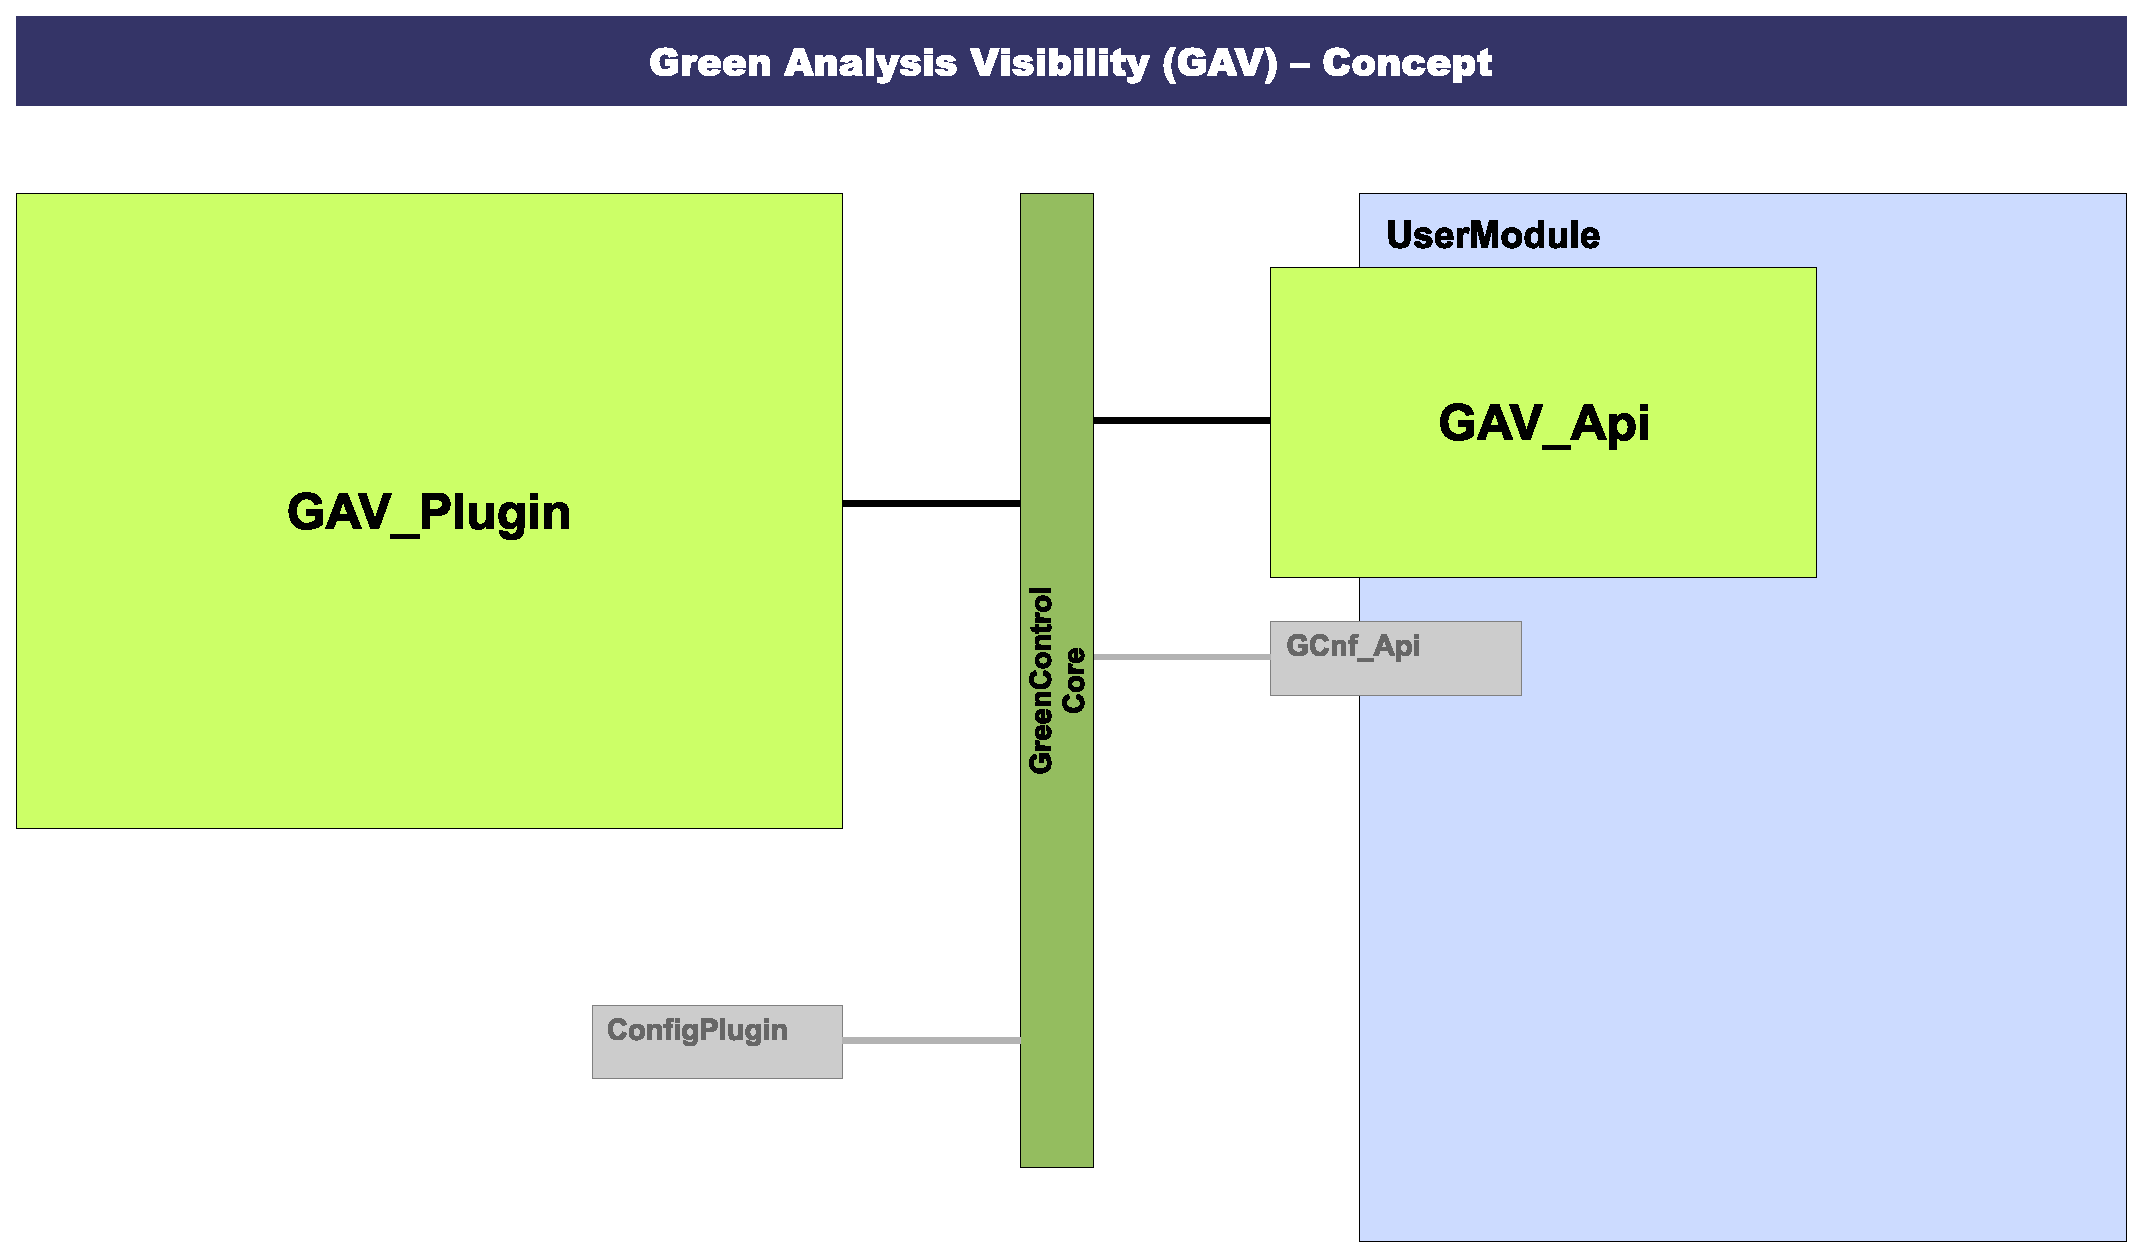
\includegraphics[width=\linewidth]{./images/GAVconcept(1)}}
	\caption{GreenAV Concept}
	\label{fig:GAVConcept1}
\end{figure}

Figure \ref{fig:GAVConcept2} is an overview over the most important elements of \GreenAV. The user module may use the \lstinline|GAV_Api| to access \lstinline|OutputPlugin|s (see section \ref{GAVOutputPlugins}). The user module also can create Statistics Calculator objects \lstinline|StatCalc| and the concerning \lstinline|Trigger|s and \lstinline|Calculator|s (see section \ref{GAVStatisticsCalculator}). The event listeners are members of the \lstinline|GAV_Plugin|. One is used by the output plugins and one is used by the triggers without the user's recognition.

\begin{figure}[ht]
	\centerline{
		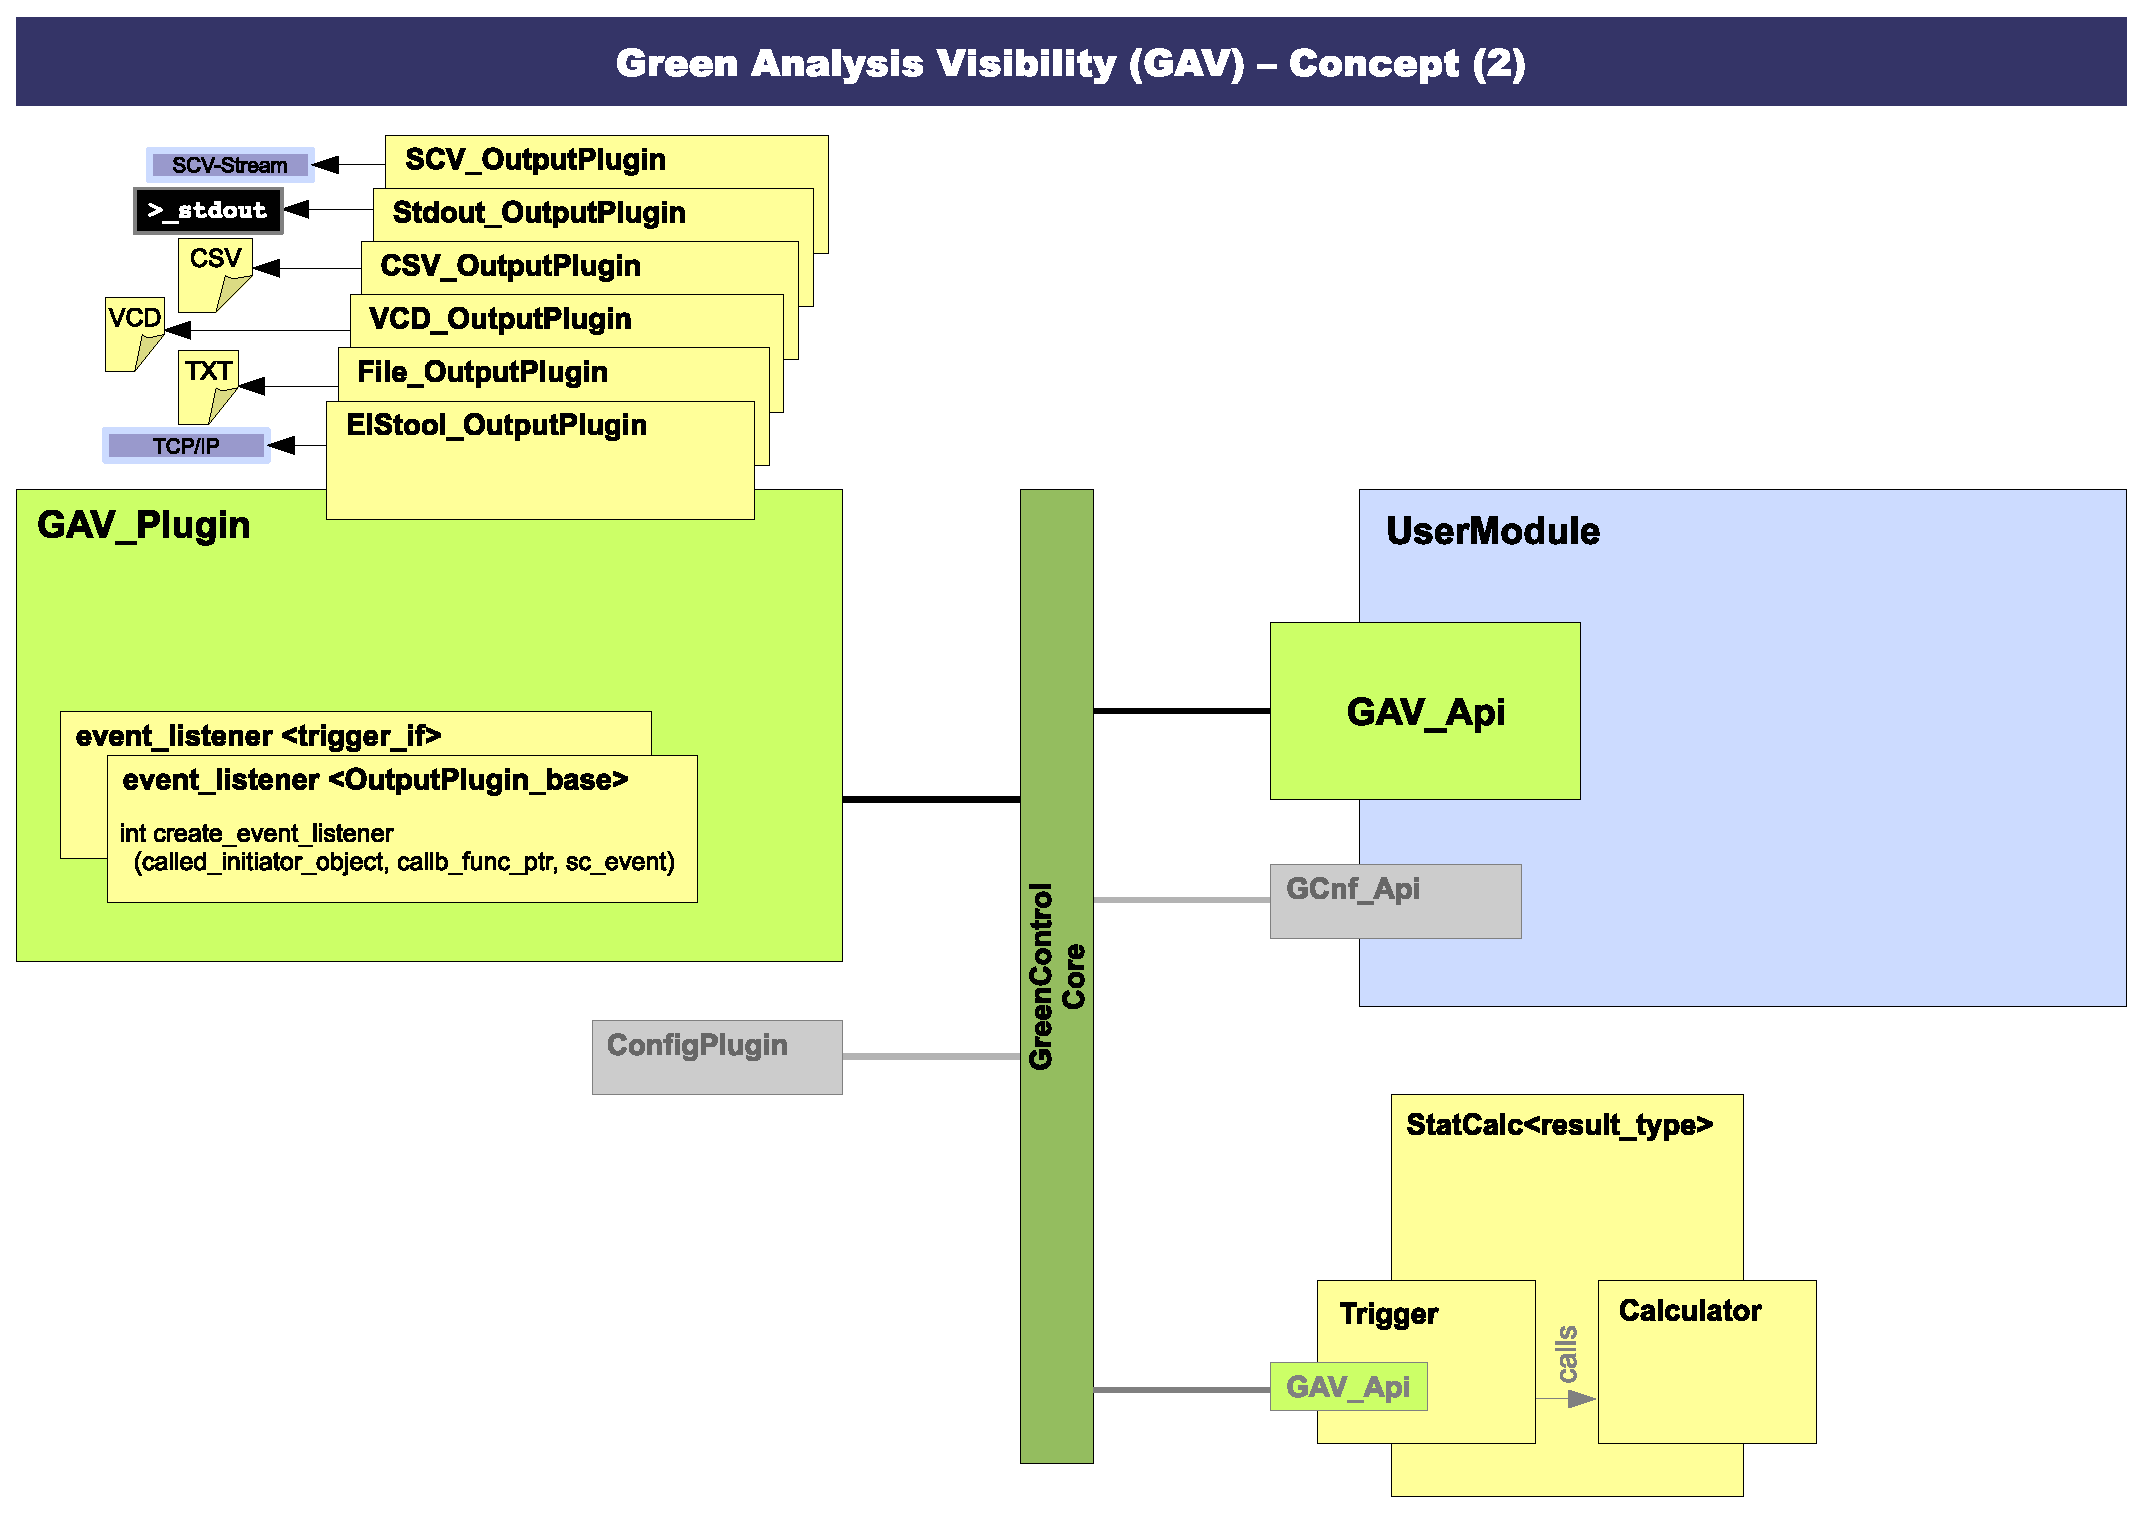
\includegraphics[width=\linewidth]{./images/GAVconcept(2)}}
	\caption{GreenAV full Concept}
	\label{fig:GAVConcept2}
\end{figure}

%%%%%%%%%%%%%%%
%%%%%%%%%%%%%%%

\section{Namespace gs::av}
\label{GAVnamespace}

All analysis and visibility classes of this \GreenAV framework are located within the namespace {\sffamily gs::av} which is a sub namespace of the GreenSocs namespace {\sffamily gs}.

This framework uses the \GreenControl namespace {\sffamily gs::ctr} and some elements of the \GreenConfig namespace {\sffamily gs::cnf}.

A \lstinline[language=TeX]|using namespace ctr;| statement in the \GreenAV global import file imports the control namespace to the {\sffamily gs::av} namespace (see \Datei{greencontrol/gav/plugin/gav\_globals.h}).

\Note{Compatibility Note}{Namespace compativility to release 0.2}{
	To be compatible to the old namespaces (tlm::gc, tlm::gc::config) the header
	file \Datei{greencontrol/namespace\_compatibility.h} can be included!
}

%%%%%%%%%%%%%%%
%%%%%%%%%%%%%%%

\section{API adapter GAV\_Api}
\label{GAVUserAPI}

This section is about the GAV user API. For a full API reference see the \hyperlink{GAVDoxygenRef08target}{doxygen API reference}. Here follows a brief description of the most important functions:


\begin{tabularx}{\textwidth}{|X|} 
  \hline
  {\sffamily create\_OutputPlugin (OutputPluginType type, string ctor\_param)} \\
  \hline
  Creates a new OutputPlugin instance of the specified type in the plugin and provides the specified constructor parameter. The constructor parameter is interpreted dependent on the output plugin type (e.g. a file name or stream name or ignored). \\
  \hline
  Returns a pointer to the output plugin. \\
  \hline
  See section \ref{GAVOutputPlugins} for details. \\
  \hline
\end{tabularx} 

\begin{tabularx}{\textwidth}{|X|} 
  \hline
  {\sffamily get\_default\_output (OutputPluginType type = DEFAULT\_OUT)} \\
  \hline
     Get the default output plugin of the specified type or the simulation-wide default.\newline
     Not specifying the OutputPluginType will return the simulation-wide default one. \\
  \hline
  Returns a pointer to the default output plugin. \\
  \hline
  See section \ref{GAVOutputPlugins} for details. \\
  \hline
\end{tabularx} 

\begin{tabularx}{\textwidth}{|X|} 
  \hline
  {\sffamily add\_to\_default\_output (OutputPluginType type, gs\_param\_base *par)} \newline 
  {\sffamily add\_to\_default\_output (OutputPluginType type, gs\_param\_base \&par)} \\
  \hline
  Adds a gs\_param to be outputted by the (implicit existing) default output plugin of the specified type. The type {\sffamily DEFAULT\_OUT} may be used to add to the simulation-wide output plugin.
   \newline 
  For each {\sffamily OutputPluginType} type there is existing one object in the GAV plugin. (The object will be created at its first usage.)  \\
  \hline
  Returns a pointer to the output plugin. \\
  \hline
  See section \ref{GAVOutputPlugins} for details. \\
  \hline
\end{tabularx} 

\begin{tabularx}{\textwidth}{|X|} 
  \hline
  {\sffamily add\_to\_output (OutputPlugin\_if* outputPluginID, gs\_param\_base *par)} \\
  \hline
  Adds a gs\_param to be outputted by the specified output plugin.\newline
  The specified output plugin has to be created by calling \lstinline|create_OutputPlugin| or has to be set by calling \lstinline|get_default_output|.  \\
  \hline
  See section \ref{GAVOutputPlugins} for details. \\
  \hline
\end{tabularx} 

\begin{tabularx}{\textwidth}{|X|} 
  \hline
  {\sffamily get\_event\_listener ()} \\
  \hline
  Returns an event listerner for triggers. \newline
  May be used for any further purposes.\\
  \hline
  See sections \ref{GAVEventListener} and \ref{GAVTrigger} for details. \\
  \hline
\end{tabularx} 


%%%%%%%%%%%%%%%
% (c) GreenSocs Ltd 2008
% author: Christian Schroeder <schroeder@eis.cs.tu-bs.de>

%%%%%%%%%%%%%%%
\section{Output Plugins}
\label{GAVOutputPlugins}

{\em Output plugins} are used to export any \lstinline|gs_param| value over time to a specific output. Such outputs can be the stdout, text-files, csv-files, vcd-files, SCV streams, dedicated connections to tools, e.g. TCP/IP connections etc. (see Figure \ref{fig:GAVConceptOutputs}).

Each output plugin is able to output multiple \lstinline|gs_param|s which can be added to the output during simulation runtime by a user or a tool. The only assumption is to have access to a GAV User API (see section \ref{GAVUserAPI}).

Before you are able to use one or more output plugin(s), you have to include the one(s) you need:

\noindent
\begin{minipage}{\textwidth}
\begin{lstlisting}[caption={Include for output plugin}, label=lst:GAVIncludeOutputPlugin]
// e.g.
#include "greencontrol/analysis.h" // includes the Standard Output Plugin
#include "greencontrol/analysis_file_outputplugin.h"
#include "greencontrol/analysis_csv_outputplugin.h"
#include "greencontrol/analysis_scv_outputplugin.h"
#include "greencontrol/analysis_vcd_outputplugin.h"
// etc.
\end{lstlisting}
\end{minipage}

\begin{figure}[htbp]
	\centerline{
		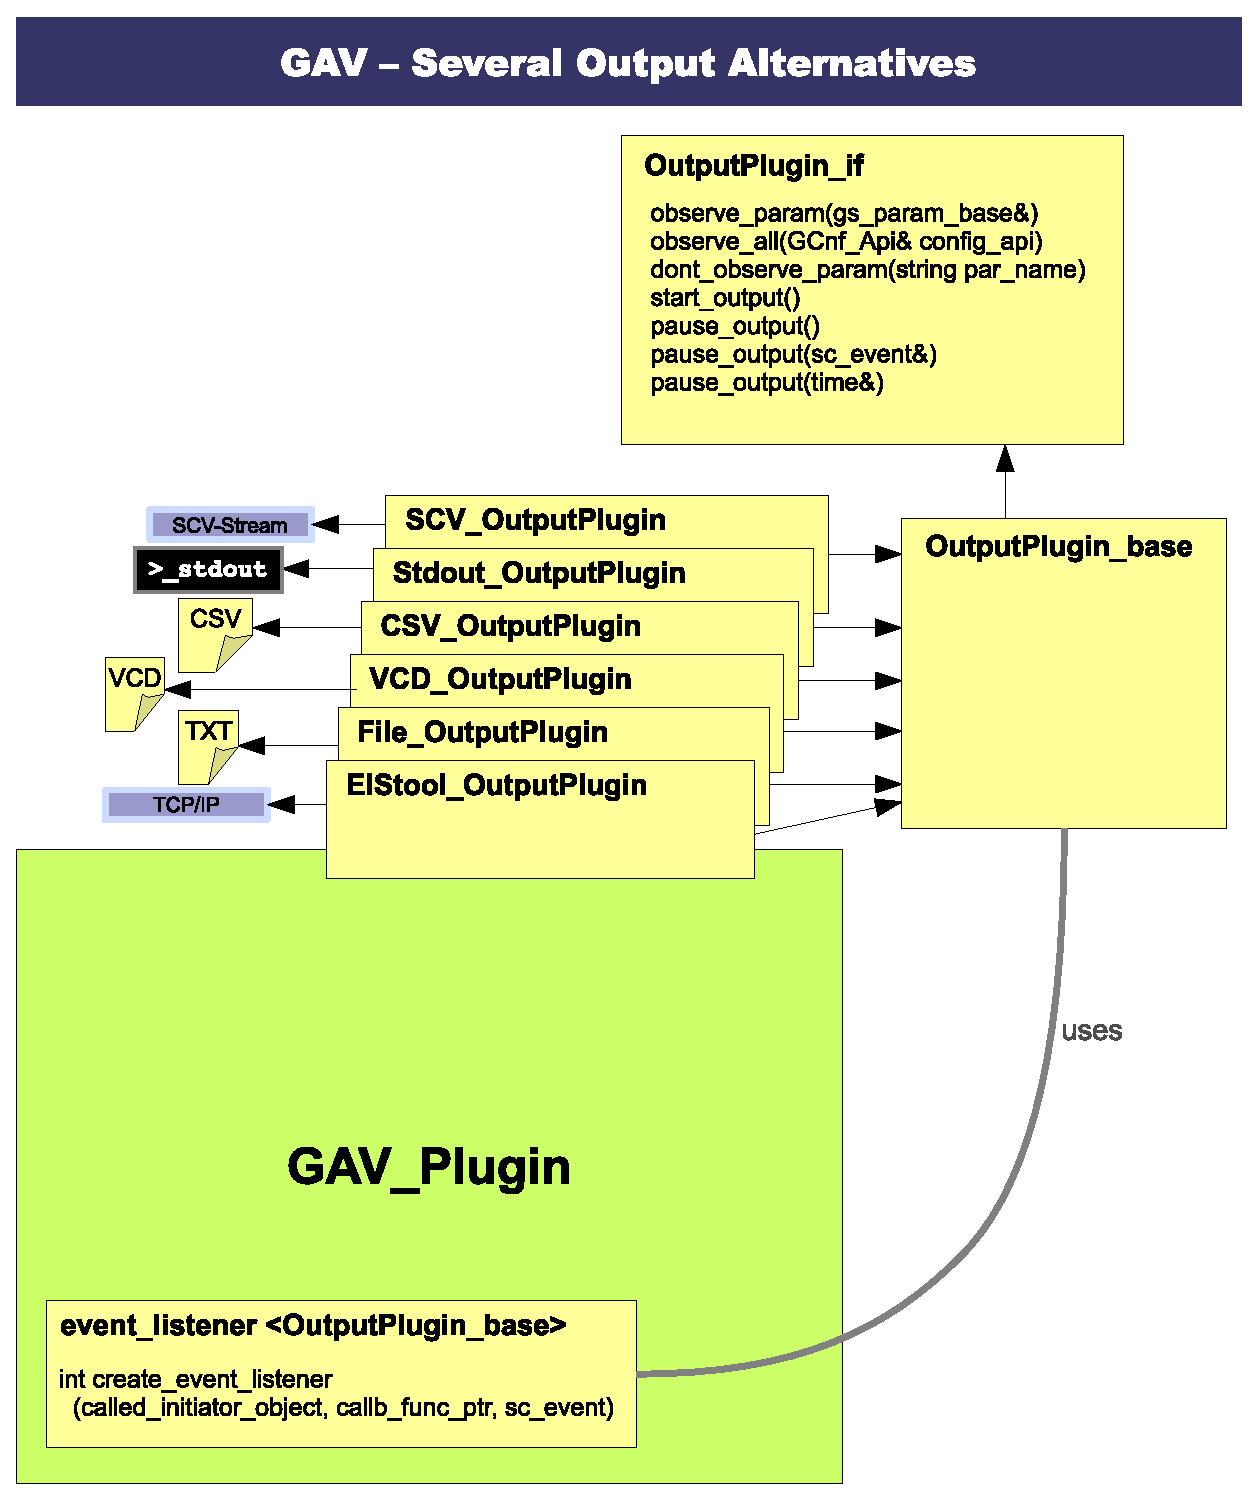
\includegraphics[width=12cm]{./images/GAVconcept(Outputs)}}
	\caption{GreenAV Concept for Outputs: The \lstinline|GAV_Plugin| contains several types of output plugins}
	\label{fig:GAVConceptOutputs}
\end{figure}


%%%
\ZwischenUberschrift{Default Output Plugin(s)} 
The provided output plugins are described in the following subsections. Any output plugin existing in the simulation is owned by the GAV plugin. For each type of output plugin there is one {\em default instance} which should be used if (only) one instance (instead of multiple ones) meets the user's requirements. A simulation-wide default output plugin type (which results in a default instance) should be set by the user during construction. If more than the default output(s) is needed (e.g. if several files should be created) the user may create {\em additional instances} of each output plugin type.

Specify the simulation-wide default output plugin like shown in listing \ref{lst:GAVDefaultOutputPlugin}. All outputs that are not directed to a special type or instance will use this default output plugin.

The output plugin types are identified with the type {\sffamily gs::gav::OutputPluginType} (which is an unsigned int). For convenience their names can be used instead. See the following sections of each output plugin for its value. {\sffamily DEFAULT\_OUT} is used as a replacement for the simulation-wide default.

\noindent
\begin{minipage}{\textwidth}
\begin{lstlisting}[caption={Specify the default output plugin during Analysis Plugin instantiation}, label=lst:GAVDefaultOutputPlugin]
gs::av::GAV_Plugin analysisPlugin(gs::av::STDOUT_OUT);
\end{lstlisting}
\end{minipage}

\WarningSymbol{} Only if you know what you are doing, you may use the GAV Plugin function \newline \lstinline[language=TeX]|void set_default_output_plugin(OutputPluginType default_output_plugin_type)| \newline
to modify the default output plugin even during model creation and simulation.

See next paragraph and section \ref{GAVUserAPI} for how to access default output plugins and how to create and access additional ones.

\Note{Implementation Note}{Output Plugin identification}{
  The output plugins are identified (id) using the {\sffamily unsigned int OutputPluginType}. A static map {\sffamily OutPluginName::getMap()} is used to store the names (values) related to the id (key).
  
  A variable of type {\sffamily OutputPluginType}, named as the output plugin name, with the corresponding value can be used to identify the type using  {\sffamily gs::av::TXT\_FILE\_OUT} etc. 
}

%%%%
\ZwischenUberschrift{Access Output Plugins}\hypertarget{AccessOutputPlugins}
Before using an output plugin the user needs to get a default instance or create a new one. Use the GAV user API (see section\ref{GAVUserAPI}). Several functions are available to access output plugins. See the code example for an example how to use.

\begin{itemize}
  \item Recommended way accessing the default output plugin of the needed type: \newline
     Get the default output plugin by calling
     \lstinline[language=TeX]|OutputPlugin_if* get_default_output(const OutputPluginType type = DEFAULT_OUT)|.
     If the module does not care about the output type, leave the type empty which will return the simulation-wide default output plugin. The returned output plugin pointer can be used to add parameters for observation or to control it (see section \hyperlink{InterfaceAndHowToUse}{Interface and how to use}).

  \item When needing further output plugin instances, a call of \lstinline|OutputPlugin_if* create_OutputPlugin (OutputPluginType, string ctor_par)| will create a new instance using the string as constructor parameter (e.g. filename). The user should store the returned pointer to be able to add parameters using the function \lstinline|add_to_output| (see below).
  
\end{itemize}


%%%%
\ZwischenUberschrift{Observing Parameters with Output Plugins}
Observing a parameter with an output plugin means that the output plugin creates output each time the observed parameter(s) change. This observation is realized using the parameter' value change (post\_write) callbacks.

There are two basically different ways adding a parameter for observation to an output plugin: One way is calling GAV user API functions. This assumes you have pointer access to the output plugin instance and the parameter (which is no issue within the simulation). Another way is creating and manipulating parameters belonging to special output plugins. For this you need to know the name of the output plugin you want to observe a parameter and the name of the parameter.

{\em Manipulate output plugins directly}:
\begin{itemize}
	\item See section \hyperlink{InterfaceAndHowToUse}{Interface and how to use} for various actions possible on output plugin pointers that you got by calling \lstinline|get_default_output| or creating new ones (see section \hyperlink{AccessOutputPlugins}{Access Output Plugins}).
\end{itemize}

Observe parameters by {\em calling GAV user API functions}:
\begin{itemize}
  \item Adding a parameter for observation to a default or manually created output plugin can be done using the function
      \mbox{\lstinline|OutputPlugin_if* add_to_output(OutputPlugin_if*, gs_param_base*)|.} The output plugin (first parameter) is one of the pointers returned by the functions above (\lstinline|get_default_output| and \lstinline|create_outputPlugin|).
  
  \item Another way observing a parameter with one of the default plugins is calling \lstinline|OutputPlugin_if* add_to_default_output(OutputPluginType, gs_param_base*)| which adds a parameter to the default instance of the specified type. It returns a pointer to the default output plugin, too.
  
  \item The easiest way observing a parameter with the simulation-wide default output is calling 
  	the function \lstinline|OutputPlugin_if* add_to_default_output(gs_param_base*)|. It returns 
	a pointer to the default output plugin, too.
\end{itemize}

Observe parameters by {\em creating and manipulating parameters belonging to special output plugins}:
\begin{itemize}
  \item To enable the observation of a parameter (which may be already existing or may not), create a new implicit parameter which is a child parameter of the output plugin and is named as the parameter that should be observed. This comes clear in the following example:
	\begin{itemize}
  		\item The GAV Plugin is named ``{\sffamily AnalysisPlugin}''.
  		\item The output plugin which should observe the parameter is the default stdout one, automatically named \mbox{``{\sffamily STDOUT\_OUT\_default}''}.
		\item The parameter that should be observed is named ``{\sffamily mymodule.submodule.myparam}''.
		\item To observe the parameter with the output plugin, simply create a so-called {\em enabled parameter} (child of the output plugin) named \mbox{``{\sffamily AnalysisPlugin.STDOUT\_OUT\_default.mymodule.submodule.myparam}''} by doing the following call on the config user API:  
		\begin{lstlisting}
mCnfApi->setInitValue("AnalysisPlugin.STDOUT_OUT_default.mymodule.submodule.myparam", "true");
		\end{lstlisting}
		The output plugin will automatically make the implicit parameter explicit immediately.
		\item Afterward you can enable and disable the observation of the parameter by modifying the 'enabled parameter' to true or false, e.g. 
		\begin{lstlisting}
gs::gs_param<bool> *enabled
  = mCnfApi->get_gs_param<bool>("AnalysisPlugin.STDOUT_OUT_default.mymodule.submodule.myparam");
*enabled = false;
		\end{lstlisting}
	\end{itemize}

This works as well with any manually created output plugin. E.g. to add a parameter to an output plugin named \mbox{``{\sffamily mymodule.main\_action.STDOUT\_OUT\_userChosenConstructorParam}''} this is done by calling
		\begin{lstlisting}
mCnfApi->setInitValue("mymodule.main_action.STDOUT_OUT_userChosenConstructorParam.mymodule.param2", "true");
		\end{lstlisting}

\end{itemize}

%%%%
\ZwischenUberschrift{Output plugin behavior}

The default behavior (which differs between different output plugins) is that after adding a parameter for observation, -- if the output plugin is running -- the first log output is caused immediately when the parameter is added. This helps logging e.g. initial values.

% Alte Nummerierung sichern
\let\oldtheenumi=\theenumi
\let\oldlabelenumi=\labelenumi
% Neue Nummerierung mit Buchstaben definieren
\renewcommand{\theenumi}{\roman{enumi}}
\renewcommand{\labelenumi}{\alph{enumi})}

%User-View:
\begin{itemize}
  \item An output plugin has the free choice to begin paused (which is \textsl{not} the desired default). In this case it is the output plugin's choice %(see below on resume())
    \begin{enumerate}
        \item to cache (desired default)
        \item or drop the changes.
    \end{enumerate}
    \begin{itemize}
      \item All output plugins get automatically started (by calling \lstinline|resume|) during end\_of\_elaboration
      \begin{itemize}
        \item To prevent an output plugin to start there, the user can call \lstinline|dont_start| before end\_of\_elaboration
      \end{itemize}
      \item The user has the option to start each output plugin by calling \lstinline|resume()| whenever he wants - that might be before the automatic start during end\_of\_elaboration or after, if e.g. \lstinline|dont_start| has been called before.
    \end{itemize}

  \item When an output plugin starts paused, calling \lstinline|resume()|
    \begin{enumerate}
          \item could output the values recorded/cached before (desired behavior)
          \item or could just start outputting.
    \end{enumerate}

  \item When \lstinline|pause()| gets called (which is not the automatic internal pause on instantiation), the o-plugin has the choice to
    \begin{enumerate}
          \item keep the callbacks but drop changes (desired default)
          \item or keep the callbacks and record/cache changes to output them on \lstinline|resume|
          \item or do a) or b) but unregister callbacks.
    \end{enumerate}
  \item When \lstinline|resume| get called during simulation, the o-plugin has the choice to
    \begin{enumerate}
          \item output the first value change (desired default)
          \item or output the current value(s)
    \end{enumerate}
\end{itemize}

\Note{Implementation Note}{Output Plugins handling callbacks}{
\begin{itemize}
    \item Base class behavior: When a parameter is added for observation, the base class will immediately call the output plugin's callback function.
    \item The callback function can use \lstinline|m_constructing| to check if called during construction.
    \item The output plugin is able to check if a call is a usual value change callback or the initial add-for-observation-call by checking the base class' member \lstinline|m_currently_calling_initial_add_for_observation_callback|.
\end{itemize}
}

\WarningSymbol{Info:} Output plugins may start paused by default because an output plugin might need to initialize \textsl{after} all parameters have been added (e.g. CSV file outputs should begin with a complete the header line containing all parameters).


%Alte Nummerierung wiederherstellen
\let\theenumi=\oldtheenumi
\let\labelenumi=\oldlabelenumi


%%%%
\ZwischenUberschrift{Output Plugin Names}
An output plugin is an {\sffamily sc\_object} which is named in the following pattern. The name is needed e.g. when creating 'enabled parameters' (see above) for this output plugin.

All output plugin names have their name string as prefix (e.g. {\sffamily STDOUT\_OUT}) and their constructor parameter as tail.

The default output plugins (one for each available output plugin type) are created and owned by the GAV Plugin. Their name tails are {\sffamily \_default} (which is the constructor parameter specified by the GAV Plugin).

The tail is automatically converted to SystemC conform names by replacing each character which is not a letter or a digit or an underscore to an underscore.

Examples:
\begin{itemize}
	\item {\em Default} output plugin of type {\sffamily STDOUT\_OUT}: \newline 
	name: {\sffamily AnalysisPlugin.STDOUT\_OUT\_default}
	\item {\em Default} output plugin of type {\sffamily TXT\_FILE\_OUT}: \newline
	name: {\sffamily AnalysisPlugin.TXT\_FILE\_OUT\_default}
	\item User created output plugin created {\em in the constructor} of module {\sffamily mymodule} with the call \lstinline|create_OutputPlugin(TXT_FILE_OUT, "myop")|: \newline
	name: {\sffamily mymodule.TXT\_FILE\_OUT\_myop}
	\item User created output plugin created {\em in the constructor} of module {\sffamily mymodule} with the call \lstinline|create_OutputPlugin(TXT_FILE_OUT, "myop.txt")|: \newline
	name: {\sffamily mymodule.TXT\_FILE\_OUT\_myop\_txt}
	\item User created output plugin created {\em in the thread} {\sffamily main\_action} of module {\sffamily mymodule} with the call \lstinline|create_OutputPlugin(TXT_FILE_OUT, "myop.txt")|: \newline
	name: {\sffamily mymodule,main\_action.TXT\_FILE\_OUT\_myop\_txt}
\end{itemize}

%%%
\ZwischenUberschrift{Interface and how to use}\hypertarget{InterfaceAndHowToUse}
After the user got an output plugin pointer of type \lstinline|OutputPlugin_if| (see \Datei{OutputPlugin\_if}) it may be used: Call

\begin{itemize}
  \item \lstinline|observe(gs_param_base&)| to let the output plugin observe a parameter.
  \item \lstinline|observe_all(GCnf_Api& config_api)| to observe all parameters currently existing.
  \item \lstinline|observe(vector<gs_param_base*>)| to observe parameters given in a vector (e.g. as a result of the config user API call \lstinline|getParams(string)|).
  \item \lstinline|observe(string getParamList_string)| to observe parameters specified by a string like \mbox{``\sffamily myModule.*}''. Internally the config API call \lstinline|getParams(string)| will be used. To observe all parameters underneath the hierarchy level of {\sffamily myModule}, call \lstinline|observe("myModule.*")|.
  \item \lstinline|remove(gs_param_base&)| to remove a parameter observation from the output.
  \item \lstinline|pause()| to pause the output from now on.
  \item \lstinline|pause(sc_event&)| to pause the output until the given event is notified.
  \item \lstinline|pause(sc_time&)| or \lstinline[language=TeX]|pause(double, sc_time_unit)| to pause the output for the given time.
  \item \lstinline|resume()| to resume the output manually if paused.
  \item \lstinline|paused()| to check if paused.
\end{itemize}

Consult the doxygen API \footnote{\hypertarget{GAVDoxygenRef08target}{\GreenAV doxygen API}: \url{http://www.greensocs.com/projects/GreenControl/GreenAV/docs/GreenAVDoxygen} (take care to look at the correct release)} for more details.

An output plugin is not paused by default.

The usage of output plugins is shown in the example \Verzeichnis{greencontrol/examples/gav\_simple}, especially in the files \Datei{AVAnalyserTool.*}.

The type of output plugins is defined with an enum {\sffamily OutputPluginType} (see file \mbox{\Datei{gav\_datatypes.h}).}

\noindent
\begin{minipage}{\textwidth}
\paragraph{Code example}
Listing \ref{lst:GAVOuputExample} and figure \ref{fig:GAVOutputExample} show examples how to use output plugins.

\begin{lstlisting}[caption={Output plugin code example}, label=lst:GAVOuputExample]
// get pointer to parameter bases
gs::gs_param_base *int_par  = m_configAPI.getPar("Owner.int_param");
gs::gs_param_base *str_par  = m_configAPI.getPar("Owner.str_param");
gs::gs_param_base *uint_par = m_configAPI.getPar("Owner.uint_param");

// get simulation-wide default output, and observe a param
gs::av::OutputPlugin_if* overallDefaultOP = m_analysisAPI.get_default_output();
m_gavApi.add_to_output(overallDefaultOP, int_par);
// alternative: add params to the default text file output  
gs::av::OutputPlugin_if* fileOP =
    m_gavApi.add_to_default_output(gs::av::TXT_FILE_OUT, int_par);
m_gavApi.add_to_default_output(gs::av::TXT_FILE_OUT, uint_par);

// create an additional CSV-file output plugin and add all existing
// parameter to output
gs::av::OutputPlugin_if* csvFileOP = 
    m_gavApi.create_OutputPlugin(gs::av::CSV_FILE_OUT, "CSVexp.log");
csvFileOP->observe_all(m_configAPI);

// pause for 2 ns.
csvFileOP->pause(2, SC_NS);

// remove parameter from default file output
fileOP->remove(*int_par);
\end{lstlisting}
\end{minipage}

\begin{figure}[ht]
	\centerline{
		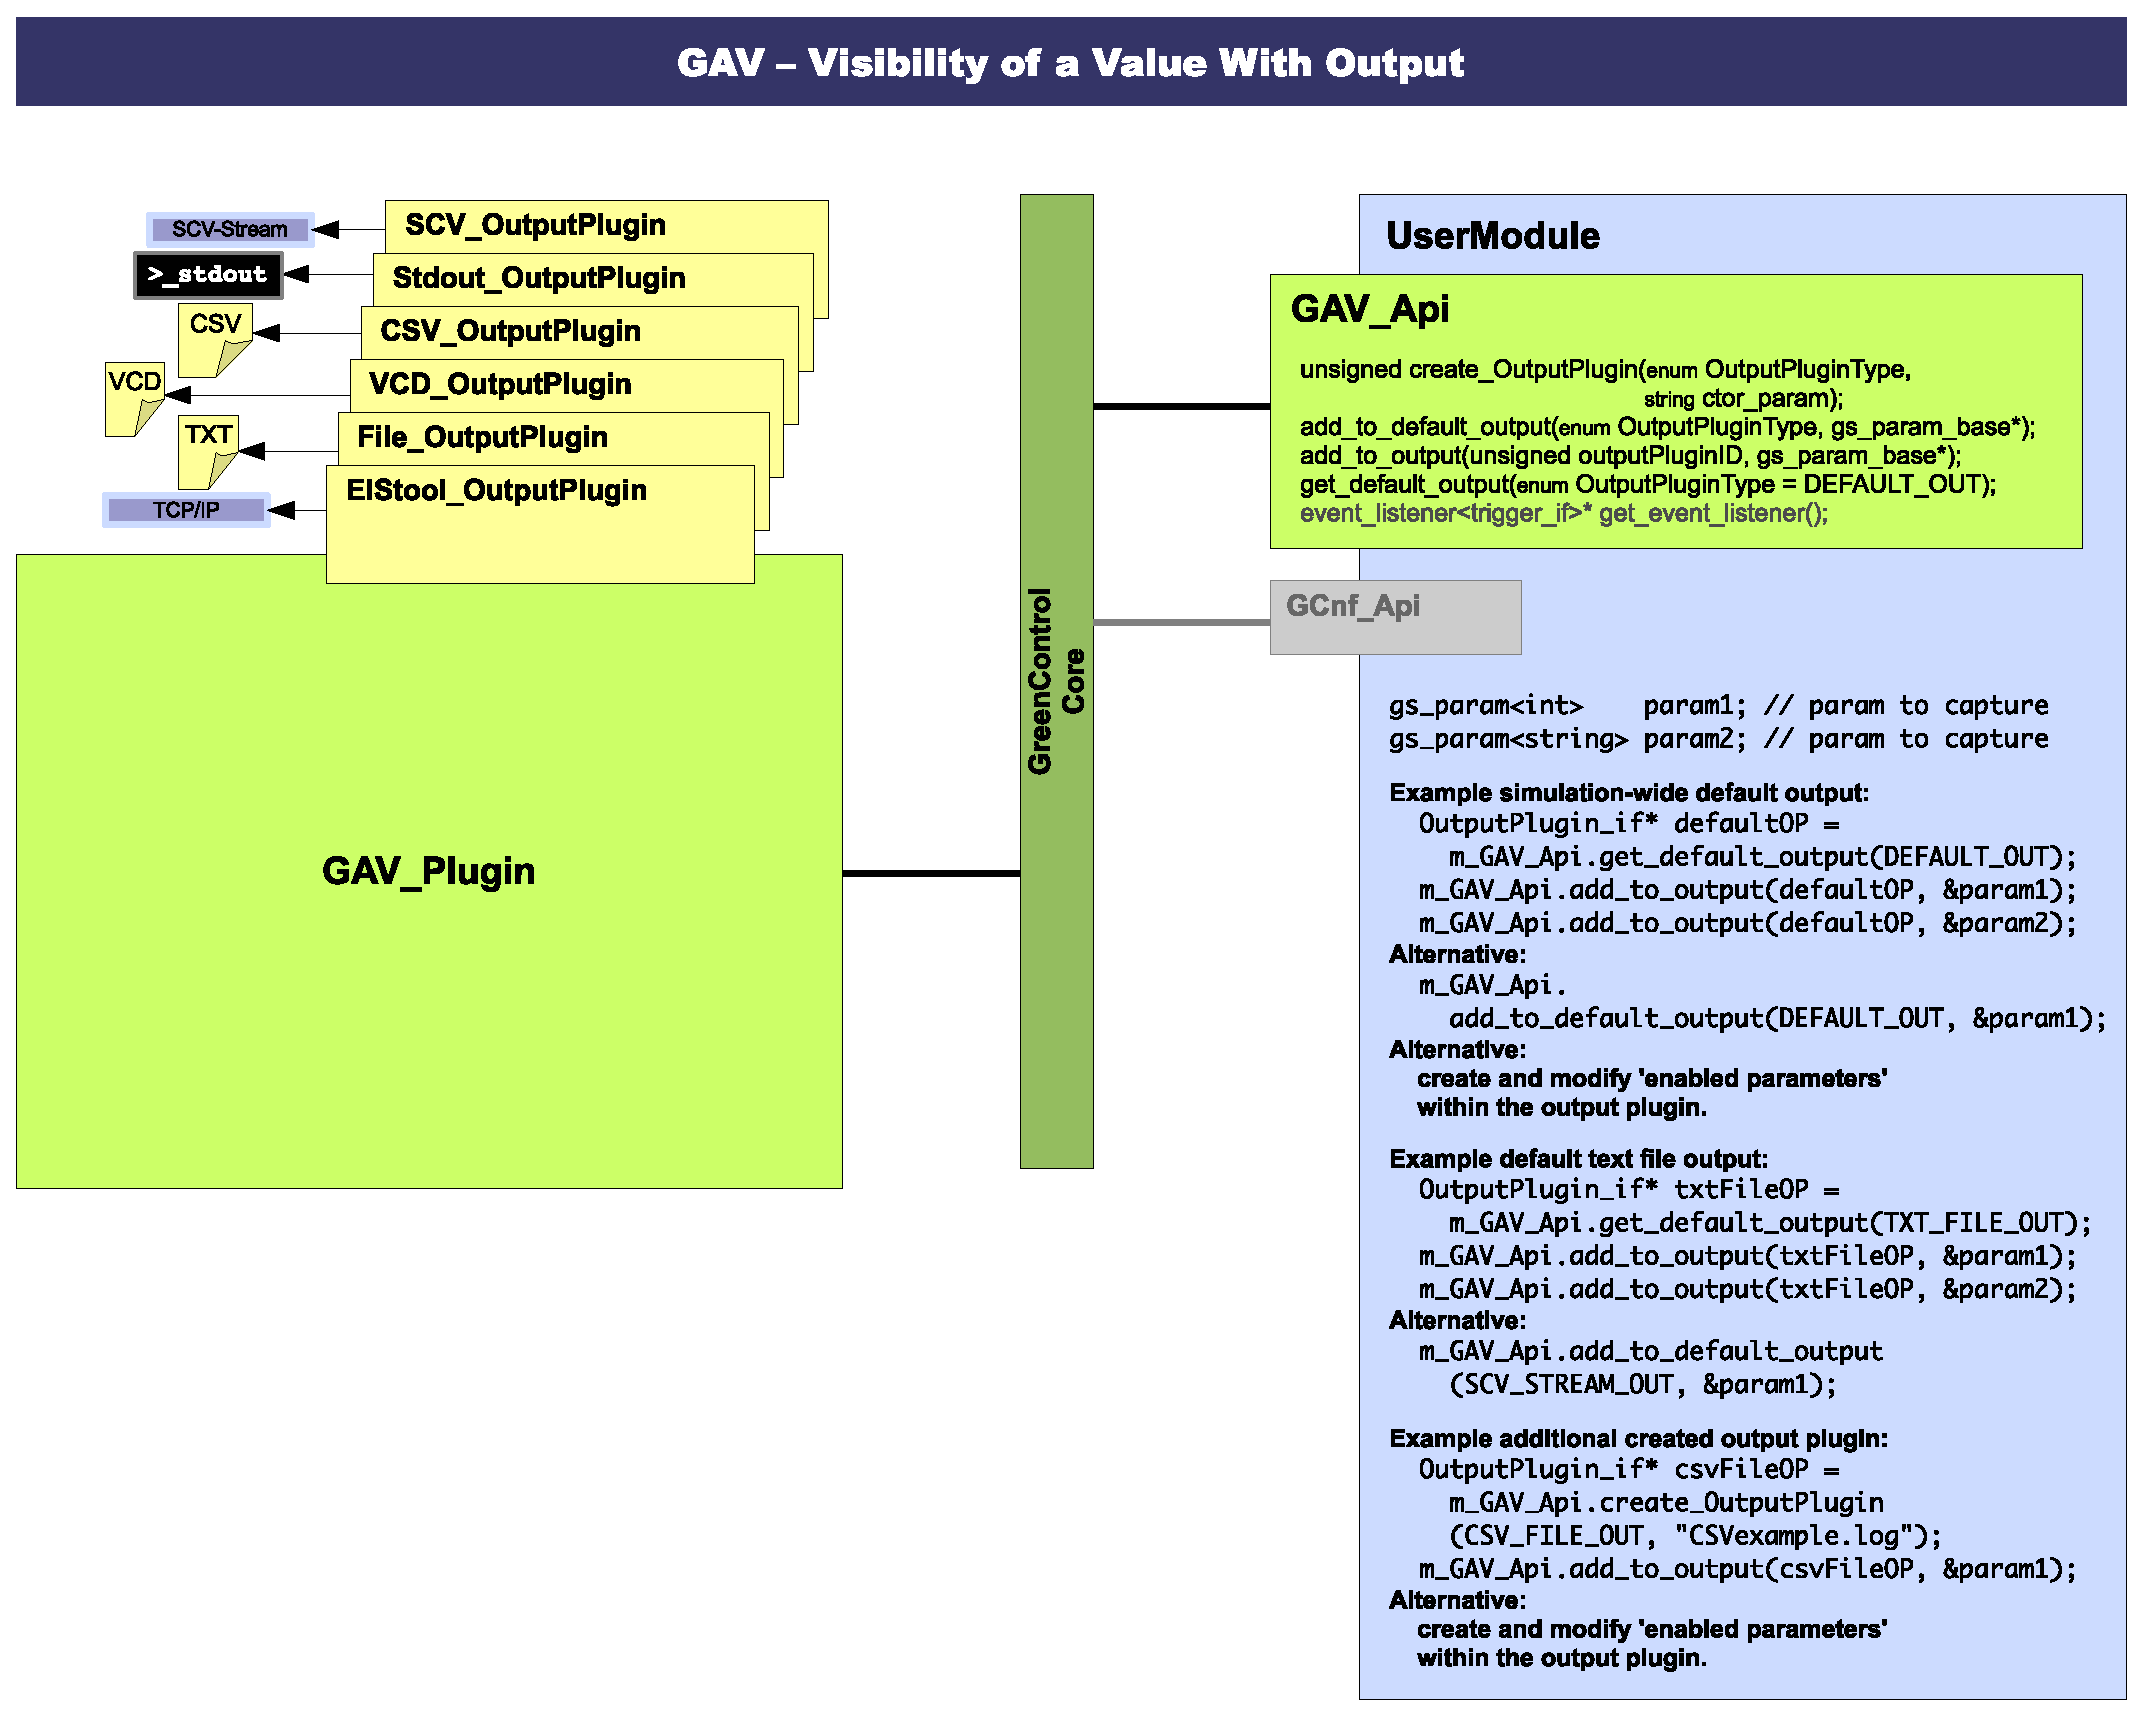
\includegraphics[width=\linewidth]{./images/GAVconcept(OutputExample)}}
	\caption{GreenAV Output Example}
	\label{fig:GAVOutputExample}
\end{figure}


\Note{Implementation Note}{Output Plugin}{
  The output plugin instances are newed by the GAV plugin and stored in two maps: one for the 
  default (\lstinline|m_DefaultOutputPlugins|) and one for the additional (\lstinline|m_OutputPlugins|) output plugins.
  
  One event listener (\lstinline|m_OutpPl_event_listener|, see section \ref{GAVEventListener}) is owned by the GAV plugin to handle events (pause and resume) of output plugins.
}

\Note{Implementation Note}{OutputPlugin\_base}{
 An output plugin derives from the base class \lstinline|OutputPlugin_base| (see file \Datei{OutputPlugin\_base}).\\

 Each output plugin needs only implement its constructor, destructor, the initialization function \lstinline|init()| and
 the callback function \lstinline|config_callback| which should perform the actual output.

 Output plugins implement the constructor which gets one string parameter
 to allow adding the output plugin to the GAV plugin's create command.
 
 All functions are virtual to give the derived class the oportunity to catch the
 calls before calling the base class' function. \\

 The derived classes' \lstinline|init()| is automatically called by the base class before the first callback access (dependent on the variable \lstinline|bool is_used|), not during construction. The constructor should not do memory allocations etc. because it is called (for the default output plugins) even if the output plugin will never be used.
}


%%%%
\subsection{Default Output Plugin (special case)}
\label{GAVOPdefault}

\begin{itemize}
  \item Identify the default output plugin (which is actually one of the following) with \newline
  	{\sffamily gs::av::DEFAULT\_OUT}, \newline
           id ({\sffamily OutputPluginType}) = 0.
\end{itemize}

%%%%
\subsection{NULL Output Plugin (special case)}
\label{GAVOPnull}

\begin{itemize}
  \item Identify the NULL output plugin (which is actually no one) with \newline
  	{\sffamily gs::av::NULL\_OUT}, \newline
           id ({\sffamily OutputPluginType}) = 1.
\end{itemize}

Use this setting if the output should go nowhere.

%%%%
\subsection{STDOUT Output Plugin}
\label{GAVOPstdout}

\begin{itemize}
  \item Included within \Datei{greencontrol/analysis.h}
  \item Implementation see file \Datei{Stdout\_OutputPlugin.h}
  \item Identify this output plugin with {\sffamily gs::av::STDOUT\_OUT}, \newline
           id ({\sffamily OutputPluginType}) = 3.
  \item Behavior:
    \begin{itemize}
        \item Starts running (needs not be started manually or automatically).
        \item Does not cache value changes when paused.
        \item On resume it outputs the first value change (not the current value).
    \end{itemize}
\end{itemize}

The STDOUT output plugin can be used to simply display parameter changes to the standard output (e.g. terminal where the simulation runs).

One line per parameter change is printed and contains timing (and delta) information, the parameter name and the new value. An output example can be seen in listing \ref{lst:stdoutOutputPluginEx}.

This output plugin is a very convenient way to print each parameter change to the simulation output.

The constructor string parameter is not used within this output plugin.

\begin{lstlisting}[caption={STDOUT output example}, label=lst:stdoutOutputPluginEx]
@130 ns /7 (Stdout_OutputPlugin): AVnewStatCalc.int_par = 2
\end{lstlisting}


%%%%
\subsection{Text-file Output Plugin}
\label{GAVOPfile}

\begin{itemize}
  \item Include \Datei{greencontrol/analysis\_file\_outputplugin.h}
  \item Implementation see file \Datei{File\_OutputPlugin}
  \item Identify this output plugin with {\sffamily gs::av::TXT\_FILE\_OUT}, \newline
           id ({\sffamily OutputPluginType}) = 2.
  \item Behavior:
    \begin{itemize}
        \item Starts running (needs not be started manually or automatically).
        \item Does not cache value changes when paused.
        \item On resume it outputs the first value change (not the current value).
    \end{itemize}
\end{itemize}

The Text-file output plugin can be used to record parameter changes to a human-readable text file. The format is similar to the STDOUT plugin's output: The first line is the simulation time, the following lines contain one line per parameter change. See listing \ref{lst:fileOutputPluginEx} for an example.

The constructor parameter is the filename of the output file. Be careful to set the file extension (e.g. {\sffamily .txt} or {\sffamily .log}). If the given file name has no extension (no dot in it) the extension {\sffamily .log} will be added automatically.

\begin{lstlisting}[caption={Text-file output example}, label=lst:fileOutputPluginEx]
Simulation time: Fri Mar 28 15:03:09 2008

@1 ns /1: Owner.int_param = 100
@1 ns /1: Owner.uint_param = 670
@1 ns /1: Owner.int_param = 101
@2 ns /3: Owner.int_param = 102
\end{lstlisting}

\paragraph{Pure Output} Pure output is a special feature of the text-file output plugin. The additional function \lstinline[language=TeX]|void pure_output(const std::string&)| can be called to write directly to the text file without waiting for parameter change callbacks and without using the formating functionality of the output plugin. This feature is used by report message streamers (see project \textsl{ReportMessages}). % TODO: Link

\begin{lstlisting}[caption={Text-file \textsl{pure} output example}, label=lst:fileOutputPluginPureEx]
std::string mystring;
mystring = "Any string to output to file"; mystring += std::endl;
gs::av::OutputPlugin_if* op 
  = m_analysisAPI->create_OutputPlugin(gs::av::TXT_FILE_OUT, "file.log");
gs::av::File_OutputPlugin* fop 
  = dynamic_cast<gs::av::File_OutputPlugin*>(op);
fop->pure_output(mystring);
\end{lstlisting}


%%%%
\subsection{Comma Separated Values (CSV) Output Plugin}
\label{GAVOPcsv}

\begin{itemize}
  \item Include \Datei{greencontrol/analysis\_csv\_outputplugin.h}
  \item Implementation see file \Datei{CSV\_OutputPlugin}
  \item Identify this output plugin with {\sffamily gs::av::CSV\_FILE\_OUT}, \newline
           id ({\sffamily OutputPluginType}) = 4.
  \item Behavior:
    \begin{itemize}
        \item Starts paused (will start automatically during end\_of\_elaboration or can be started manually).
        \item Does not cache value changes when paused.
        \item On resume it outputs the first value change (not the current value).
    \end{itemize}
\end{itemize}

The Comma Separated Values (CSV) output plugin can be used to output parameter changes that should be imported to MS Excel.

The constructor parameter of the \lstinline|CSV_OutputPlugin| is the filename of the output file. The default filename (for the plugin's default output plugin) is {\sffamily default.csv}. If the filename string has not the postfix '{\sffamily .csv}' this will be appended automatically.

    Due to the structure of CSV files all parameters must be registered before
    writing the file! The plugin will begin writing the file on the first parameter change.

    The behavior how to react to newly added parameters after began writing can be
    adapted with the \lstinline[language=TeX]|#define ALLOW_ADDING_PARAMETERS_AFTER_HEADER_WRITTEN|.
    If not defined the output plugin will refuse (ignore) all register requests 
    for new parameters after having written the first value! If defined the output
    plugin will add this new observed parameter to each following line. Accordingly
    the row witdh may increase within the CSV-file - which is imported by Excel without
    problems. But the head of the table will \emph{not} include the parameter name, 
    the last columns will remain unnamed!
   
    Pausing the plugin does {\em not} write the current time slot to the file because the
    plugin may be resumed again during the same time slot.

    The separator character can be specified with the macro \lstinline[language=TeX]|#define SEPARATOR ';'|.
    For standard-conform CSV-files this separator has to be a \lstinline[language=TeX]|','|, 
    for files to be imported by Excel \lstinline[language=TeX]|';'| should be used (default).
    
    The following text file is an example for a file created by this plugin. The first line is the time of the simulation run, the thirs line is the output name (constructor parameter, file name), the fifth line is the header of the table containing the parameter names. All remaining lines are data (parameter changes). This example includes integer and string parameters. Figure \ref{fig:GAVcsvExcelExample} shows the file opened with Excel.

\noindent
\begin{minipage}{\textwidth}
\begin{lstlisting}[language=TeX, caption={CSV output file example}]
Simulation time: Fri Mar 28 14:00:42 2008

CSVexample.log
 
"time /delta";"Owner.int_param";"Owner.str_param";"Owner.uint_param";
"1 ns /1";"101";"Hello World!";"670"
"2 ns /3";"104";;
"2 ns /4";"106";"Hello Germany!";
"2 ns /5";;"Hello Arizona!";
"2 ns /6";;"Hello France!";
"3 ns /7";;;"2000"
"5 ns /8";"222";"new hello";"3000"
"106 ns /10";"133";;
"210 ns /18";"10000";;
\end{lstlisting}
\end{minipage}

\begin{figure}[htbp]
	\centerline{
		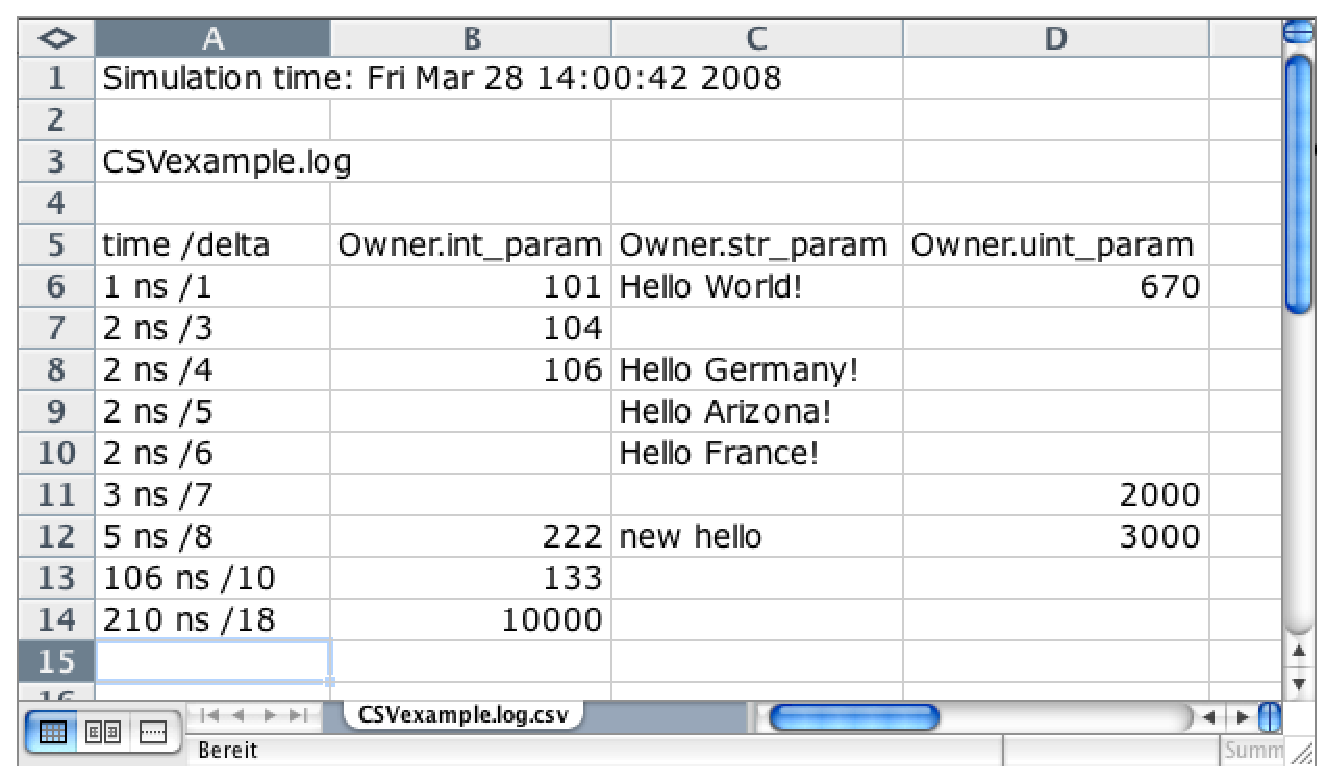
\includegraphics[width=15cm]{./images/csvExcelExample}}
	\caption{CSV ouput plugin Excel example}
	\label{fig:GAVcsvExcelExample}
\end{figure}


%%%%
\subsection{SCV-stream Output Plugin}
\label{GAVOPscv}

\begin{itemize}
  \item Include \Datei{greencontrol/analysis\_scv\_outputplugin.h}
  \item Implementation see file \Datei{SCV\_OutputPlugin}
  \item Identify this output plugin with {\sffamily gs::av::SCV\_STREAM\_OUT}, \newline
           id ({\sffamily OutputPluginType}) = 5.
  \item Behavior:
    \begin{itemize}
        \item Starts running (needs not be started manually or automatically).
        \item Does not cache value changes when paused.
        \item On resume it outputs the first value change (not the current value).
    \end{itemize}
\end{itemize}

The SCV output plugin (\lstinline|SCV_OutputPlugin|) outputs parameter changes to a stream of the SystemC Verification Standard (SCV). This standard stream can be used as an input to several vendor tools (such as CoWare and Mentor).

 This output plugin exports the registered
 parameter changes to an {\em SCV stream} named \mbox{\sffamily GreenAVstream\_$<$OutputPluginName$>$}. The constructor string parameter is the {\sffamily OutputPluginName}. Each
 parameter gets its own transaction generator. When a parameter changes, the previous
 transaction is ended and a new one with the new value is started. Accordingly a 
 transaction represents the time where the value of a parameter remains unchanged.

 The database that should be written to can be chosen in the static function 
 \lstinline|init_scv_recording()| (see file \Datei{SCV\_OutputPlugin.h}).

The output plugin's {\em default database} is a text file which is the default database in the SCV framework. The SCV stream output is written to the file \Datei{transaction\_text\_db}.  Add \#define areas to use other databases (like ModelSim).

There are some options to change the output plugin's behavior to be able to support a wide range of external tools reading the SCV stream. These options can be changed in the define area at the top of the file \Datei{SCV\_OutputPlugin.h}.

\begin{itemize}

  \item  The default is to use only one globals database for all SCV output plugin instances. If there is a database type that is able to handle more than one database, undefine the \newline
  \lstinline[language=TeX]|#define ONLY_ONE_GLOBAL_DATABASE|.

  \item  If a tool or database is only able to handle one stream, use the \lstinline[language=TeX]|#define ONLY_ONE_GLOBAL_STREAM| (defined by default). \newline
 Then all \lstinline|SCV_OutputPlugin| instances write to the same stream.

  \item  The OutputPlugin is able to create transactions with values of the type {\sffamily string} (default)
 The user may set \lstinline[language=TeX]|#define USE_CORRECT_TYPE_TRANSACTIONS true|
 to enable transactions containing values of the correct type (as long as the type is listed in the enum
 {\sffamily gs::cnf::Param\_type} and is implemented here). This is slower because of 
 some additional switch statements and casts.

\end{itemize}

The files \Datei{AVscvAnalyserTool.*} in the example \Verzeichnis{greencontrol/examples/gav\_simple} create SCV output streams.


\ZwischenUberschrift{Experience with Mentor Graphics ModelSim}
{\sffamily ModelSim} (Mentor Graphics) has the ability to run SystemC simulations and to show the results graphically. GreenBus and \GreenControl (including \GreenConfig and \GreenAV) can be compiled with Mentor's {\sffamily sccom} compiler and can be run with the {\sffamily vsim} simulator.

Mentor's SCV implementation does not support string data types in transactions being recorded in an SCV stream. Accordingly the SCV output plugin has to use the {\sffamily \small USE\_CORRECT\_TYPE\_TRANSACTIONS} define and cannot show string parameters. So the visualization is restricted to the data types listed in the enumeration {\sffamily gs::cnf::Param\_type} and implemented in the plugin.

The SCV output plugin has an \lstinline|init_recording| function which automatically uses ModelSim special code when compiled with the ModelSim sccom compiler. In the define section there is an \lstinline|ifdef| for ModelSim which automatically sets the correct behavior.
  
These steps have to be performed when simulating with ModelSim:
\begin{itemize}
  \item Start the simulation ({\em Important!} The transaction stream does not occur before simulation is running and has created the stream!)
  \item View the recorded SCV transactions by right clicking on the module which contains the stream and selecting {\sffamily Add $\rightarrow$ Add All Signals to Wave}. %(TODO: This should be the GAV plugin named 'AnalysisPlugin' but is is the module which initiated the first observation of this output plugin.) 
\end{itemize}


\ZwischenUberschrift{Experience with CoWare}
Experiments with the {\sffamily CoWare Platform Architect}:

To use the CoWare settings, \#define \lstinline|CoWare|. The SCV output plugin has a special define area in its \lstinline|init_recording| function for the CoWare tool. In the define section there is an \lstinline|ifdef| for CoWare which automatically sets the correct behavior.


%%%%
\subsection{Value Change Dump (VCD) Output Plugin}
\label{GAVOPvcd}

\begin{itemize}
  \item Include \Datei{greencontrol/analysis\_vcd\_outputplugin.h}
  \item Implementation see file \Datei{VCD\_OutputPlugin.h}
  \item Identify this output plugin with {\sffamily gs::av::VCD\_FILE\_OUT}, \newline
           id ({\sffamily OutputPluginType}) = 6.
  \item Behavior:
    \begin{itemize}
        \item Starts paused (will start automatically during end\_of\_elaboration or can be started manually).
        \item Does not cache value changes when paused.
        \item On resume it outputs the first value change (not the current value).
    \end{itemize}
\end{itemize}

The Value Change Dump (VCD) output plugin can be used to output
parameter changes that can be viewed graphically using a VCD viewer
like GTKWave.

The constructor parameter of the \lstinline|VCD_OutputPlugin| is the
filename of the output file. The default filename (for the plugin's
default output plugin) is {\sffamily default.vcd}. If the filename
string has not the postfix '{\sffamily .vcd}' it will be appended
automatically.

Due to the structure of VCD files all parameters must be registered
before the first write of the file. The plugin will start paused and
begin writing the file when resumed, either automatically durig
end\_of\_elaboration or manually by calling the \lstinline|resume()|
method. New parameter additions will cause an error.

Figure \ref{fig:GAVvcdGTKWave} shows an example of a file created by
this plugin (from example gav\_simple) and opened with GTKWave. Note
that the plugin has support for text strings (str\_param in the
figure). To show a wave as a text in GTKWave, select Edit / Data
Format / ASCII. The parameters int\_param and uint64\_param are shown
in Decimal data format.

\begin{figure}[htbp]
	\centerline{
		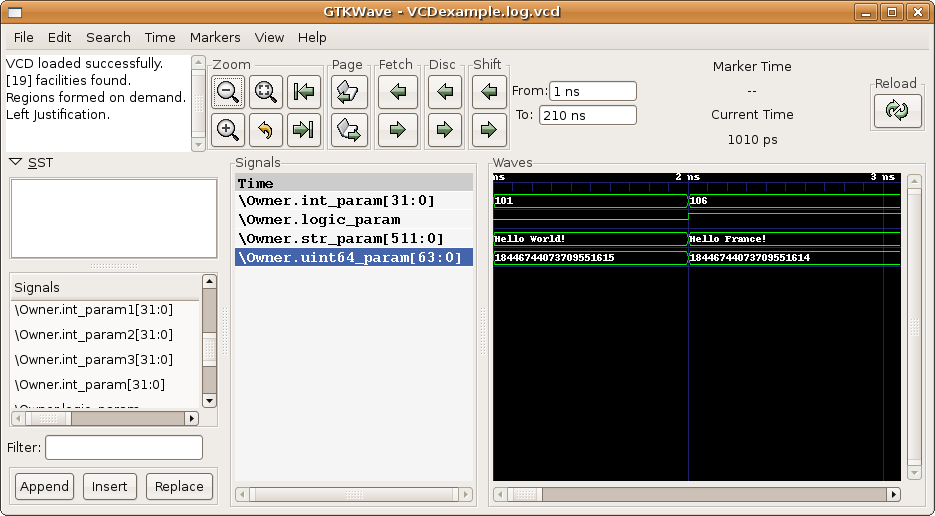
\includegraphics[width=17cm]{./images/vcdGTKWave}}
	\caption{VCD output file showed in GTKWave}
	\label{fig:GAVvcdGTKWave}
\end{figure}


%%%%
\subsection{How to implement an Output Plugin}
\label{GAVimplementOP}

This is a short introduction how to implement a new output plugin. For a simple example see the STDOUT output plugin in file \Datei{Stdout\_OutputPlugin.h} (see section \ref{GAVOPstdout}).

\begin{itemize}
  \item Outside the class (but in same namespace) specify the project-wide unique id and convenience name with the macro {\sffamily GAV\_REGISTER\_PLUGIN(unique\_id, convenience\_variable, class\_name)}. \newline
     Example:
    \begin{lstlisting}
GAV_REGISTER_PLUGIN(10, MY_NEW_OUT, MyNew_OutputPlugin);
    \end{lstlisting}
  \item Inherit \lstinline|OuputPlugin_base| which provides most functionality expect the output itself.
  \item Do not implement the empty constructor.
  \item Implement the constructor taking a name and an event listener and forward them to the base class including the project-wide convenience name and the output plugin's starting behavior:
    \begin{lstlisting}
MyNew_OutputPlugin ( const char* output_specifier, 
                     event_listener<OutputPlugin_base> *ev_listn)
 : OutputPlugin_base(output_specifier, ev_listn, 
                     convenience_variable, start_running)
    \end{lstlisting}
  \item Implement the callback function and make sure to remove a parameter being observed by the output plugin when is is being destroyed. Guard the output by checking \lstinline|is_running|.
    \begin{lstlisting}
void config_callback(gs_param_base &par) {
  if (par.is_destructing()) {
    remove(par);
  }  else if (is_running) {
    // Do the output
  }
}
    \end{lstlisting}
    Optionally use the base class members \lstinline|m_constructing| and \lstinline|m_currently_calling_initial_add_for_observation_callback| if needed.
  \item Implement the output within the callback function (previous bullet point). Use the functions the \lstinline|gs_param_base| provides or cast to the actual \lstinline|gs_param<type>| type (see \GreenConfig User's Guide\footnote{\hypertarget{GCnfUsersGuide08target}{\GreenConfig User's Guide}: \url{http://www.greensocs.com/projects/GreenControl/GreenConfig}}).
    \begin{lstlisting}
par.getName();
par.getString(); 
    \end{lstlisting}
  \item Create a member representing the new output plugin in the enum {\sffamily OutputPluginType} in file \Datei{gav\_datatypes.h}.
    \begin{lstlisting}
enum OutputPluginType {
  [... other members ...],
  // Short explanation of my outp.pl.
  MYNEW_OUTPUT_PLUGIN
}
    \end{lstlisting}
  \item Add the new output plugin to the GAV plugin's \lstinline|outputPluginFabricCreator| function (file \Datei{gav\_plugin.h}) by adding a switch case. The case is the enum member being created at the preceding bullet point.
    \begin{lstlisting}
case MYNEW_OUTPUT_PLUGIN:
{
  // create MyNew output plugin
  op = new MyNew_OutputPlugin(constructParam, &m_OutpPl_event_listener);
  break;
}
    \end{lstlisting}
  \item See the code documentation (Doxygen API reference or header files) for some more detailled information.


\end{itemize}

\Note{Advanced Note}{Write an Output Plugin from scratch}{
  When writing a completely new output plugin at least the interface {\sffamily OuputPlugin\_if} has to be implemented. The constructor should get (but needs not) the string given by the user, transmitted over the transaction.
}



%%%%%%%%%%%%%%%
\section{Analysis and Visibility Service}
\label{GAVService}


%%%%
\subsection{Service Plugin}
\label{GAVServicePlugin}

The service plugin (class \lstinline|GAV_Plugin|, file \Datei{gav\_plugin.h}) uses the enum member {\sffamily AV\_SERVICE} and the port plugin name {\sffamily GAV\_Plugin}.

The main functionality of the plugin:
\begin{itemize}
  \item  Manage output plugins (see section \ref{GAVOutputPlugins}),
  \item  Own two event listeners needed by output plugins and Statistics Calculator Triggers (see sections \ref{GAVOutputPlugins} and \ref{GAVStatisticsCalculator}).
\end{itemize}



%%%%
\subsection{Commands}
\label{GAVCommands}

The analysis and visibility service {\sffamily AV\_SERVICE} uses the command enum {\sffamily GAVCommand} (see file \Datei{gav\_datatypes.h}).

These commands may be used for the API -- Plugin communication:

\noindent
\begin{tabularx}{\textwidth}{|p{5.1cm}|X|}
	\cline{1-1}\cline{2-2}\multicolumn{2}{|l|}{  Direction:  \newline API $\rightarrow$ GAV Plugin    }\\ 
	\cline{1-1}\cline{2-2} {\bf Command}    &  Usage   \\ 
	\cline{1-1}\cline{2-2} \lstinline|CMD_ADD_TO_OUTPUT_PLUGIN|    &   
		Adds a parameter to an output plugin. The output plugin can be either the default one of the 
		specified type or a user API specified one. If the default one is being used for the first time 
		the output plugin will be instantiated by the plugin. \\ 
	\cline{1-1}\cline{2-2} \lstinline|CMD_CREATE_OUTPUT_PLUGIN|    &   
		Creates a new output plugin of the specified type and returns the pointer to the API.  \\ 
	\cline{1-1}\cline{2-2} \lstinline|CMD_GET_EVENT_LISTENER|    &   
		Returns the pointer to the plugin's trigger event listener to the API.  \\ 
	\hline
\end{tabularx}

The fields of the transaction are used for special commands on this way:\newline
\noindent
\begin{tabularx}{\textwidth}{|p{3.3cm}|p{2.3cm}|p{2cm}|X|}
	\cline{1-1}\cline{2-2}\cline{3-3}\cline{4-4} Command                &  Phase       &  Field             &  Description   \\ 
	\cline{1-1}\cline{2-2}\cline{3-3}\cline{4-4} \lstinline|CMD_ADD_TO_ OUTPUT_PLUGIN|&  REQUEST     &  
		{\em AnyPointer}    &  $!= NULL$: 'Identifier' (pointer) of the output plugin the parameter should be added to.
		\newline $== NULL$: add to the default output plugin.  \\ 
	\cline{1-1}\cline{2-2}\cline{3-3}\cline{4-4}                        &  REQUEST    &  {\em AnyUint}       & 
		If ({\em AnyPointer} $== NULL$): type of the default output plugin 
		(member of enum {\sffamily OutputPluginType}).  \\ 
	\cline{1-1}\cline{2-2}\cline{3-3}\cline{4-4}                        &  REQUEST    &  {\em AnyPointer2} & 
		Optional: Pointer (void*) to the parameter that should be added. \newline
		$== NULL$: and if $AnyPointer == NULL$: only return the default output plugin pointer without observing a parameter \\ 
	\cline{1-1}\cline{2-2}\cline{3-3}\cline{4-4}                        &  RESPONSE  &  {\em AnyPointer} & 
		Pointer ('identifier') to the output plugin the parameter was added. 
		Can be used in this command for adding further parameters. \newline 
		$= NULL$: on error. \\ 
	\cline{1-1}\cline{2-2}\cline{3-3}\cline{4-4}                        &  RESPONSE  &  {\em Error}       & 
		 $>0$ when adding fails.   \\ 
	\hline
\end{tabularx}

\vspace{1 cm}

\noindent
\begin{tabularx}{\textwidth}{|p{3.3cm}|p{2.3cm}|p{2cm}|X|}
	\cline{1-1}\cline{2-2}\cline{3-3}\cline{4-4} Command                &  Phase       &  Field             &  Description   \\ 
	\cline{1-1}\cline{2-2}\cline{3-3}\cline{4-4} \lstinline|CMD_CREATE_ OUTPUT_PLUGIN| &  REQUEST & {\em AnyUint}       &  
		Type of the OutputPlugin that should be created 
		(member of enum {\sffamily OutputPluginType}). \\ 
	\cline{1-1}\cline{2-2}\cline{3-3}\cline{4-4}                        &  REQUEST    &  {\em Value} & 
		Constructor parameter (string) that should be given to the output plugin's constructor 
		(containing e.g. filename dependent on the output plugin type). \\ 
	\cline{1-1}\cline{2-2}\cline{3-3}\cline{4-4}                        &  RESPONSE  &  {\em AnyPointer} & 
		Pointer ('identifier') to the created output plugin. Can be used in the 
		{\sffamily CMD\_ADD\_TO\_OUTPUT\_PLUGIN} command for adding parameters. \\ 
	\cline{1-1}\cline{2-2}\cline{3-3}\cline{4-4}                        &  RESPONSE  &  {\em Error}       &  
		No error specified so long.   \\ 
	\hline
\end{tabularx}

\vspace{1 cm}

\noindent
\begin{tabularx}{\textwidth}{|p{3.3cm}|p{2.3cm}|p{2cm}|X|}
	\cline{1-1}\cline{2-2}\cline{3-3}\cline{4-4} Command                &  Phase       &  Field             &  Description   \\ 
	\cline{1-1}\cline{2-2}\cline{3-3}\cline{4-4} \lstinline|CMD_GET_ EVENT_LISTENER| &  RESPONSE  &  {\em AnyPointer} &
		Pointer to the plugin's trigger event listener. \\ 
	\cline{1-1}\cline{2-2}\cline{3-3}\cline{4-4}                        &  RESPONSE  &  {\em Error}       &  
		No error specified so long.   \\ 
	\hline
\end{tabularx}


%%%%
\subsection{Event Listener}
\label{GAVEventListener}

Some analysis objects have to wait for events. These objects may not be allowed to be an sc\_module because they may be created during simulation runtime (e.g. the trigger of the statistics calculator, see section \ref{GAVTrigger}). To be able to wait for \lstinline|sc_event|s anyway, that object may use {\em event listeners}.

Event listeners are sc\_modules owned by the plugin doing dynamically spawned event waits: An event listener is is templated to the initiator who wants to wait for an event. When the initiator calls \lstinline|create_event_listener| the listener dynamically spawns a process being sensitive for the given event. When the event is notified the initiator is called back by the listener process.

The plugin has two event listeners:\newline
\lstinline|event_listener<trigger_if>| and \lstinline|event_listener<OutputPlugin_base>|. The one for triggers can be accessed using the GAV user API by calling \lstinline|get_event_listener| (see section \ref{GAVUserAPI}).

The listener pointer templated to \lstinline|trigger_if| can be transported to the API via a transaction of command type {\sffamily \small CMD\_GET\_EVENT\_LISTENER}. The listener templated to \lstinline|OutputPlugin_base| is used by the plugin itself when instantiating output plugins.


%%%%%%%%%%%%%%%
% (c) GreenSocs Ltd 2008
% author: Christian Schroeder <schroeder@eis.cs.tu-bs.de>

%%%%%%%%%%%%%%%
\section{Statistics Calculator}
\label{GAVStatisticsCalculator}

\ZwischenUberschrift{Concepts}
Most analysis tasks are performed by the {\em Statistics Calculator} (StatCalc) which is realized in the class \lstinline|StatCalc| in file \Datei{StatCalc.h}. The Statistics Calculator (class \lstinline|StatCalc|) manages the analysis of several 
input parameters that are calculated in a formula on several activation events. 
The tasks and the corresponding interfaces can be classified as follows:

\begin{enumerate}
  \item \textbf{Calculation Interface} (Calculator)\samepage
    \begin{itemize}
      \item Math operations
      \item Logical operations for boolean expressions usable as activation event
    \end{itemize}

  \item \textbf{Calculation Activation Events} (Trigger)
  \begin{itemize}
    \item Per default the result is updated (re-calculated) each time one of the {\em formula (input) parameter} changes.
    \item A boolean condition can guard the calculation. \newline 
    The calculation will only be performed if the given parameter is true. Note: A change of the condition parameter from false to true does not trigger re-calculation.
    \item A (complex) boolean expression can be created using another Statistics Calculator object giving its bool result parameter to \lstinline[language=TeX]|set_condition(gs_param<bool>&)|.
    \item An {\sffamily sc\_event} can be used to trigger the calculation. Each time the event is notified the calculation will be performed. (If there is a boolean condition activated this will be checked first.)
    \item A fixed interval, which triggers re-calculation each given time, can be specified.
    \item The calculation can also be manually performed by a simple function call.
  \end{itemize}

  \item \textbf{Statistics Abilities} (Calculator)
  \begin{itemize}
    \item {\em Sliding window}: The user can insert a sliding window between the calculation and the result. The sliding window puts out the average over the last $n$ values to the result parameter. \newline
    All activation mechanisms keep the same (parameter change callbacks, boolean conditions, {\sffamily sc\_event}, interval).
  \end{itemize}
\end{enumerate}

\begin{figure}[htbp]
	\centerline{
		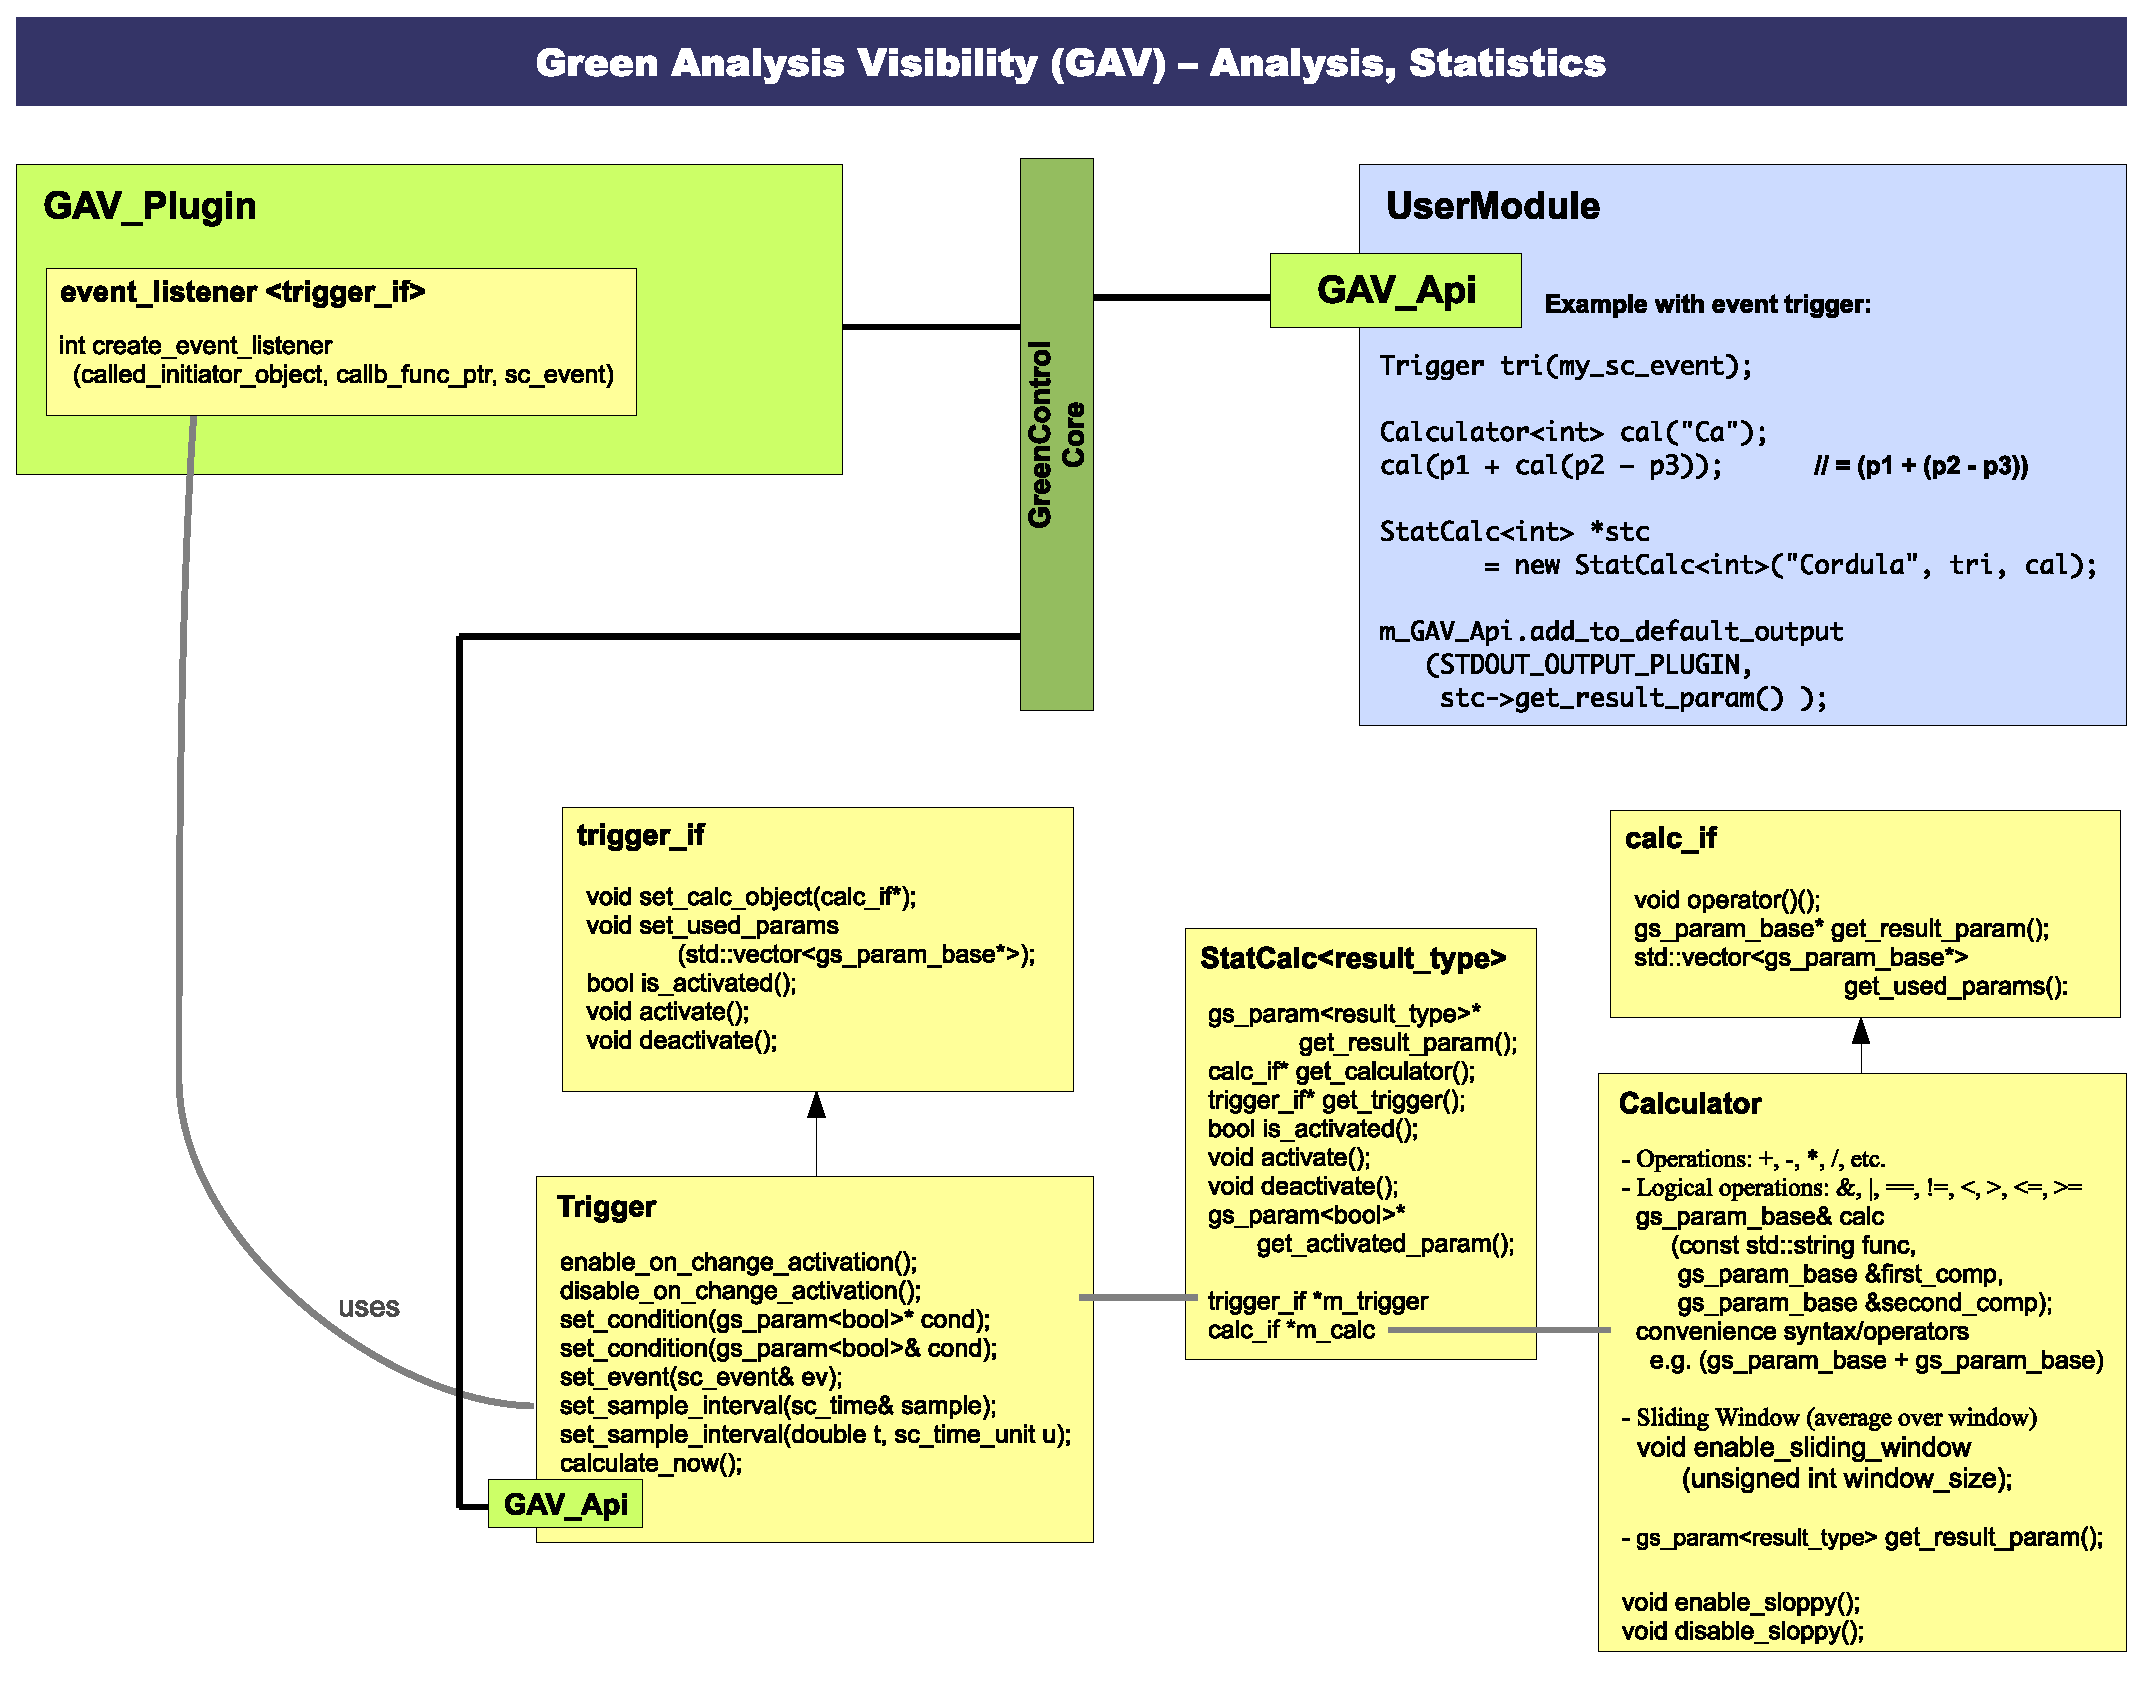
\includegraphics[width=\linewidth]{./images/GAVconcept(StatCalc)}}
	\caption{GreenAV Statistics Calculator Concept}
	\label{fig:GAVConceptStatCalc}
\end{figure}

Figure \ref{fig:GAVConceptStatCalc} shows the {\em Statistics Calculator concept}. The StatCalc consists mainly of a trigger object (see section \ref{GAVTrigger}) and a calculator object (see section \ref{GAVCalculator}). The calculator is responsible for managing the formula that should be calculated. The trigger manages the activation events of re-calculation and then calls the calculator to perform re-calculation.

The StatCalc object gets a trigger and a calculator object during construction and combines them. It gives the calculator functor object to the trigger object to enable the trigger to activate the recalculation. The StatCalc calls \lstinline|get_used_params()| on the calculator to give all input parameters to the trigger (using \lstinline|set_used_params()|.

\ZwischenUberschrift{Interface and how to use}
The \lstinline|StatCalc| object has to be instantiated {\em after} the trigger and calculator have been created and specified completely.

The {\em name} of the StatCalc has to be specified during construction and is made unique by the constructor using \lstinline|sc_gen_unique_name|.

The full constructors are:
\begin{lstlisting}
StatCalc(const char* stcalc_name, 
                        trigger_if* any_trigger, calc_if* any_calculator);
StatCalc(const char* stcalc_name, 
                        trigger_if& any_trigger, calc_if& any_calculator);
\end{lstlisting}

Alternative constructors do not need a trigger to be specified. In this case the default trigger object will we created by the StatCalc. The default trigger triggers on each input parameter change.
\begin{lstlisting}
StatCalc(const char* stcalc_name, calc_if* any_calculator);
StatCalc(const char* stcalc_name, calc_if& any_calculator);
\end{lstlisting}

The StatCalc object gives access to the trigger and calculator object pointers via the functions \lstinline|trigger_if* get_trigger()| and \lstinline|calc_if* get_calculator()| and provides some of the trigger and calculator interface functions whose calls will be redirected to the trigger object:
\begin{lstlisting}
gs_param<result_type>* get_result_param(); // redirected to calculator
calc_if* get_calculator(); // local
trigger_if* get_trigger(); // local
bool is_activated(); // redirected to trigger
void activate();     // redirected to trigger
void deactivate();   // redirected to trigger
\end{lstlisting}

The activation status of the trigger can also be accessed and manipulated with the parameter \mbox{\sffamily $<$statcalc\_name$>$.activated} which is returned by the function:
\begin{lstlisting}
gs_param<bool>* get_activated_param(); // local
\end{lstlisting}



%%%%%%%
\subsection{Trigger}
\label{GAVTrigger}

\ZwischenUberschrift{Concept}
The trigger is responsible for activation events. When one event occurs, the re-calculation of the calculator functor has to be called so the trigger object triggers the calculation. 

The trigger is an object that must inherit \lstinline|trigger_if| to allow it to be managed by the StatCalc object.

\ZwischenUberschrift{Interface}
All trigger classes have to implement the virtual interface \mbox{\lstinline|trigger_if|.} The following listing lists the functions to be implemented by a trigger class:

\noindent
\begin{minipage}{\textwidth}
\begin{lstlisting}[caption={Trigger interface trigger\_if}]
class trigger_if {
  virtual ~trigger_if() { }
  // Initialization functions
  virtual void set_activated_param(gs::gs_param<bool> &activated) = 0;
  virtual void set_calc_object(calc_if*) = 0;
  virtual void set_used_params(std::vector<gs_param_base*>) = 0;
  // User functions
  virtual bool is_activated() = 0;
  virtual void activate() = 0;
  virtual void deactivate() = 0;
  // Callback functions
  virtual void event_callback() = 0;
  virtual void interval_callback() = 0;
};
\end{lstlisting}
\end{minipage}

For a detailed description see the \hyperlink{GAVDoxygenRef08target}{API reference}.

The initialization functions are called by the StatCalc during its construction.

The function \lstinline|set_activated_param| gets a reference to the parameter that has been created by the StatCalc and which represents and modifies the activation status. The trigger has to register a callback for this parameter to react on changes. This function is called before the other initialization functions to ensure that the parameter is available.

The function \lstinline|set_used_params| gets the formula parameters of the calculator. These parameters have to be observed by the trigger for destruction. After one of these parameters has been destructed the trigger must never again call the re-calculation of the calculator!

The function \lstinline|deactivate| should deactivate the trigger until the function \lstinline|activate| is called. A deactivated trigger should unregister all input parameter callbacks (for changes and destruction checks) due to performance reasons: A deactivated trigger should produce no overhead! This allows creation of (deactivated) Statistics Calculators without runtime overhead. Get if the trigger is activated by calling \lstinline|is_activated|.

The functions \lstinline|event_callback| and \lstinline|interval_callback| are both functions that can be registered by the trigger to the event listener of the GAV plugin (which may be accessed via the \lstinline|GAV_Api|) which is templated to \lstinline|trigger_if|.

\Note{Advanced Note}{Re-implement a trigger}{
  As an extension to the \GreenAV framework new triggers can be implemented. They just have to implement the \lstinline|trigger_if| interface.
  
  This may be needed if further activation events are needed that are not met by the default \GreenAV trigger.
  
  When re-implementing a trigger be careful never calling the re-calculation if one of the formula parameters has been destroyed. Also take care to deactivate the trigger completely when the deactivation function is being called. On activation you have to check whether all formula parameters are still existing.
}

\ZwischenUberschrift{GreenAV default Trigger and calculation activation events}

The default {\em GreenAV trigger} object class is \lstinline|Trigger|.

The trigger automatically registers for callbacks of all formula (input) parameters which are given to the trigger via the \lstinline|set_used_params| call. The trigger handles destructed input parameters by deactivating the trigger forever and never again calling the calculator functor object. Even if parameter changes are not a calculation activating event, the trigger registers for callbacks just to check if the changed parameter is being destructed.

\textbf{Calculation activation event kinds} this Trigger supports are:
\begin{itemize}
  \item sc\_event for {\em SystemC events}: \vspace{.5em} \newline 
  The sc\_event calculation activation event uses the trigger event listener of the GAV plugin to wait for the user-given event. When the event is notified the trigger will be called back (function \lstinline|event_callback|) by the event trigger.

  \item sc\_time for {\em periodical sample intervals} (periodically repeated events)  \vspace{.5em} \newline 
  The sc\_time calculation activation event notifies the trigger itself periodically after the specified time intervals. This trigger also uses the API's event listener. This may be used e.g. for sliding windows that record on fixed time intervals.
  
  \item {\em value changes} on input parameters (uses parameter callbacks)  \vspace{.5em} \newline 
  This is the {\em default} trigger mechanism. The trigger registers callbacks for all formula input parameters and triggers re-calculation an each callback.
  
  \item {\em manually chosen parameter changes}
   The user may give any gs\_params to the trigger whose value changes will result in a re-calculation. These parameters need not (but may) be formula parameters.
  
  \item {\em manually}  \vspace{.5em} \newline
  The user may manually trigger the re-calculation with a simple function call.
\end{itemize}

\textbf{Additionally} the Trigger supports a
\begin{itemize}
  \item {\em Guard} ({\em no} activation event): \lstinline[language=TeX]|gs_param<bool>| for a condition to be checked before calculation.  \vspace{.5em} \newline 
  This guard parameter is checked each time the trigger got one of the activation events. If the guard's value is {\sffamily true} the re-calculation is performed, otherwise re-calculation is suppressed.
\end{itemize}

The trigger is able to handle several activation events concurrently. The user may enable value change activation and e.g. set one (or more) sc\_event(s) on whose notification triggering will also be performed. Manually triggering is always possible (taking account of the guard as well).

\Note{Implementation Note}{Event listener}{
  The trigger needs the API's event listener templated to \lstinline|trigger_if|. During construction the trigger gets a \lstinline|GAV_Api| instance and calls \lstinline|get_event_listener| and stores the pointer. 
  \vspace{.5em}

  Afterwards the trigger calls \lstinline|m_event_listener->create_event_listener(this, &trigger_if::event_callback, ev);| where it is needed to create a dynamically spawned process that waits for the event \lstinline|ev|.
}

\ZwischenUberschrift{How to use}
This section is about how to prepare the trigger in the user's code before giving it to the \lstinline|StatCalc| object.

The specific constructors specify the way the trigger waits for calculation activation events. The vector parameter takes manually chosen parameters. There are constructors for many combinations of activation events:
\begin{lstlisting}[caption={Trigger constructors with several calculation activation events and guard}]
explicit Trigger();
explicit Trigger(sc_event& event);
explicit Trigger(sc_event* event);
explicit Trigger(sc_time ti);
explicit Trigger(double t, sc_time_unit u);
explicit Trigger(bool on_changes);
explicit Trigger(sc_event& event, gs_param<bool> &cond);
explicit Trigger(sc_time &ti, gs_param<bool> &cond);
explicit Trigger(double t, sc_time_unit u, gs_param<bool> &cond);
explicit Trigger(bool on_changes, gs_param<bool> &cond);
explicit Trigger(gs_param<bool> &cond);
explicit Trigger(gs_param<bool> *cond);
explicit Trigger(sc_event &ev, sc_time &ti, bool on_changes, 
                 gs_param<bool> cond);
explicit Trigger(sc_event &ev, sc_time &ti, gs_param<bool> &cond);
explicit Trigger(sc_event &ev, sc_time &ti);
explicit Trigger(sc_event &ev, bool on_changes);
explicit Trigger(sc_time &ti, bool on_changes, gs_param<bool> &cond);
explicit Trigger(sc_time &ti, bool on_changes);
explicit Trigger(std::vector<gs_param_base*>);
\end{lstlisting}

The constructor activation event and guard order is: 
{\sffamily sc\_event}, {\sffamily sc\_time}, {\sffamily bool\_on\_changes}, {\sffamily guard}.

There may be activation event combinations which are not available, e.g. when combining manually chosen parameters with other event.Then the user may use one constructor and one of the following functions after construction: 
\begin{itemize}
  \item \lstinline|set_event(sc_event& ev)| enables trigger for SystemC events.  \vspace{.5em} \newline
    When called repeatedly all events are valid. Removing events is not possible.
  \item \lstinline|set_sample_interval(sc_time& sample)| enables periodical sample interval trigger.  \vspace{.5em} \newline
    When called repeatedly the last interval is the valid one.
  \item \lstinline|enable_on_change_activation()| enables trigger for value changes,  \vspace{.5em} \newline
    \lstinline|disable_on_change_activation()| may be used to disable the value change trigger while the trigger 'runs'.
  \item \lstinline[language=TeX]|set_condition(gs_param<bool>* cond)| or \lstinline[language=TeX]|set_condition(gs_param<bool>& cond)| sets the guard parameter.   \vspace{.5em} \newline
    \lstinline|cond = NULL| removes the guard. \newline
    When being called repeatedly the old guard will be overwritten.
\end{itemize}
All these functions may be called anytime (even if trigger already 'runs').
 
Further available functions are:
\begin{itemize}   
  \item \lstinline|calculate_now()| triggers the re-calculation manually. This call takes account of the activation and the guard just like all activation events do. 
  \item \lstinline[language=TeX]|bool is_activated()| returns if the trigger / StatCalc is activated, see interface description above.
  \item \lstinline[language=TeX]|void activate()| activates the trigger / StatCalc, see interface description above.
  \item \lstinline[language=TeX]|void deactivate()| deactivates the trigger / StatCalc, see interface description above.
  \item \lstinline[language=TeX]|void set_activation_status(bool _activate)| calls \lstinline|activate| or \lstinline|deactivate|.
\end{itemize}

The following listings are some usage examples:

For the example this predefinitions are needed:
\begin{lstlisting}
#include "greencontrol/analysis.h"
\end{lstlisting}

\vspace{.5cm}

\begin{lstlisting}[caption={Example: standard value change trigger.}]
gs::av::Trigger *stc_tom_t = new Trigger(true);
  // is the same as 
gs::av::Trigger *stc_tom_t = new Trigger();
\end{lstlisting}

\begin{lstlisting}[caption={Example: standard value change trigger with condition guard.}]
gs::gs_param<bool> condition("condition");
gs::av::Trigger stc_regina_t(condition); // uses param changes and a guard
'... create calculator, StatCalc ...'
'... do something ...'
// disable standard value change trigger
stc_regina_t.disable_on_change_activation();
'...'
stc_regina_t.calculate_now(); // calculate manually
'...'
stc_regina.deactivate(); // deactivates the trigger
'...'
stc_regina.activate(); // re-activates the trigger
\end{lstlisting}

\begin{lstlisting}[caption={Example: SystemC event trigger.}]
sc_event event0;
gs::av::Trigger stc_cordula_t(event0);
'...'
event0.notify(); // will trigger
\end{lstlisting}

\begin{lstlisting}[caption={Example: periodical sample interval trigger.}]
gs::av::Trigger stc_bob_t(10, SC_NS);
'...'
stc_bob_t.set_sample_interval(0, SC_NS); // removes trigger
\end{lstlisting}

See files \Datei{AVnewStCalc.*} in the example \Verzeichnis{greencontrol/examples/gav\_StatCalc/} for regression tests on the trigger.




%%%%%%%
\subsection{Calculator}
\label{GAVCalculator}


%%%
\ZwischenUberschrift{Concept}
The calculator functor object is responsible for performing the calculation defined by the user.
The calculator is an object that inherits \lstinline|calc_if| to allow to be managed by the StatCalc object. It performs the calculation when the \lstinline[language=TeX]|operator()| is called by the trigger.

The default {\em GreenAV calculator} object class is \lstinline|Calculator|. 


%%%
\ZwischenUberschrift{Interface}
As an extension to the \GreenAV framework new calculators can be implemented which just have to implement the virtual interface \lstinline|calc_if|:
 
\noindent
\begin{minipage}{\textwidth}
\begin{lstlisting}[caption={Calculator interface calc\_if}]
class calc_if {
  virtual ~calc_if() { }
  void operator()() = 0;
  gs_param_base* get_result_param() = 0;
  std::vector<gs_param_base*> get_used_params() = 0;
};
\end{lstlisting}
\end{minipage}

For a detailed description see the \hyperlink{GAVDoxygenRef08target}{API reference}.

The function \lstinline|operator()| enables the calculator object to be a functor. This function performs the calculation regardless of the formula input parameter status. The trigger has to make sure not to call the function if the calculation will fail (e.g. because of destructed formula parameters).

The function \lstinline|get_result_param| returns a pointer to the result parameter. The result parameter is created and owned by the calculator. This function should not be called before the formula was specified.

The function \lstinline|get_used_params| is called by the StatCalc during construction and returns all formula input parameters to be given to the trigger. These parameters are needed by the trigger for checking the destruction callbacks and -- if activated -- for the parameter change callbacks.

\Note{Advanced Note}{Re-implement a calculator} {
  As an extension to the \GreenAV framework new calculators can be implemented. They just have to implement the \lstinline|calc_if| interface.
  
  This may be needed if other calculations shall be available, e.g. calculate within a script language instead using SystemC~/~C++. If only further functions consuming two parameters are needed, user defined functions can be added to the default \GreenAV calculator, see below.
}


%%%
\ZwischenUberschrift{GreenAV default Calculator}
The default {\em GreenAV calculator} object class is \lstinline|Calculator| (and \lstinline|Calculator_bit|).

\textbf{Features} of the Calculator:
\begin{itemize}
  \item Variable data type of the Calculator's result and intermediate results:  \vspace{.5em} \newline
  	The template parameter of the Calculator class specifies the type of all operations, intermediate 
	results and the result parameter. All formula parameters will be casted to this type for each operation.
  \item Formulas with various, nested operations can be built with formula input parameters \newline
	(of type \lstinline|gs_param<T>|):
	\begin{itemize}
	  \item Math operations 
		\colorbox{hellgrau}{$+$}, \colorbox{hellgrau}{$-$}, \colorbox{hellgrau}{$/$}, \colorbox{hellgrau}{$*$},
	  \item Logical operations
	  	\colorbox{hellgrau}{$==$}, \colorbox{hellgrau}{$!=$}, \colorbox{hellgrau}{$>=$}, 
		\colorbox{hellgrau}{$<=$}, \colorbox{hellgrau}{$<$}, \colorbox{hellgrau}{$>$},
	  \item Bitwise operations 
	  	\colorbox{hellgrau}{$\&$}, \colorbox{hellgrau}{$|$} 
		(in the derived class \lstinline|Calculator_bit|), \vspace{.5em} \newline
	           \WarningSymbol{} Some data types are not allowed to have bitwise operations, accordingly 
	           they are not included in the \lstinline|Calculator| class. If these operations should be used, 
	           use the class \lstinline|Calculator_bit| instead!
	\end{itemize}
  \item Calc-syntax (\lstinline|calc(string, gs_param<T>, gs_param<T>)|) for flexible and powerful 
  	formula creation: \vspace{.5em} \newline
	This is the main part of the calculator: the mechanism to specify formulas. Use the string 
	to specify the operation, the input parameters may be results of another calc-call. 
	Calls to \lstinline|calc| can be nested.
  \item Convenient operators \colorbox{hellgrau}{$+$}, \colorbox{hellgrau}{$-$}, 
  	\colorbox{hellgrau}{$/$}, \colorbox{hellgrau}{$*$} 
	(less flexible and powerful but better human-readable) for parameter bases: \vspace{.5em} \newline
	The convenient operators may be used to replace the calc-syntax for the math operations. 
  \item User defined functions for calc-syntax: \vspace{.5em} \newline
  	It is simple to add user defined functions including their operation strings to a Calculator of 
	specified type. This may be done e.g. in the {\sffamily sc\_main}. A function added to 
    \lstinline|Calculator<type>| is also available in \lstinline|Calculator_bit<type>|.
  \item Constants in formula:  \vspace{.5em} \newline
  	Using the calc-syntax hard-coded constants may be used instead of parameters.
  \item Statistics: sliding window: \vspace{.5em} \newline
  	The sliding window can be activated after the formula has been specified completely. The sliding window gets a window size ($n$). The function will add the results of the last $n$ calculations and divide this by the window size $n$.
  \item Switch to allow {\em sloppy calculations}:  \vspace{.5em} \newline
  	A special feature of the \GreenAV Calculator is the ''sloppy'' functionality.
	The user may enable sloppy behavior to pretend runtime errors, e.g. when dividing by zero. Each 
	operation may define a default return value if sloppy is enabled. E.g. if sloppy is enabled the division
	(\colorbox{hellgrau}{$/$}) operation returns $0$ if divided by zero.
\end{itemize}

The Calculator's formula parameters are {\em limited} to these POD and SystemC {\em data types}: \newline
   \lstinline[language=TeX]|int|,
   \lstinline[language=TeX]|unsigned int|,
   \lstinline[language=TeX]|bool|,
   \lstinline[language=TeX]|double|,
   \lstinline[language=TeX]|float|,
   \lstinline[language=TeX]|unsigned long long|,
   \lstinline[language=TeX]|unsigned char|,
   \lstinline|sc_int_base|,
   \lstinline|sc_int|,
   \lstinline|sc_uint_base|,
   \lstinline|sc_uint|,
   \lstinline|sc_signed|,
   \lstinline|sc_bigint|,
   \lstinline|sc_unsigned|,
   \lstinline|sc_biguint|.  \newline
The data types are identified by the parameter call \lstinline|getType| which returns the type as an enum {\sffamily gs::cnf::Param\_type}, see file \Datei{gcnf\_datatypes.h}.

If parameters of type \lstinline|sc_time| should be used as input parameters, a Calculator of type \lstinline[language=TeX]|double| should be used.

The Calculator does {\em no} initial calculation when being created! This assures that only when the specified activation events occur the calculation will be performed.

%%%
\ZwischenUberschrift{How to use}
The steps before adding a calculator to the StatCalc's constructors are:
\begin{enumerate}
  \item Create a \lstinline|Calculator| (or \lstinline|Calculator_bit|) object giving a name to the constructor.
  \item Specify the formula which this calculator should use. Use the calc-syntax or the convenient operators.
  \item Optional: get the result parameter. This may also be called on the StatCalc object after having created it.
\end{enumerate}

%%
\paragraph{Calc-syntax}
The {\em calc-syntax} is the designated way of setting up a complex formula of several formula input parameters. A \lstinline|calc|-call gets as function call parameters a string specifying the operation and two input parameters of type \lstinline|gs_param<T>| or \lstinline|gs_param_base|. Nested calls of \lstinline|calc| function calls may be used because the \lstinline|calc| function returns an intermediate result parameter. 

The listings \ref{lst:GAVCalcEx1} and \ref{lst:GAVCalcEx2} show examples how to specify a calculation formula using the calc-syntax.

\noindent
\begin{minipage}{\textwidth}
\begin{lstlisting}[caption={
	Simple example using the calc-syntax: \newline 
	Calculator type: {\sffamily unsigned long long}, formula: $(scint + scbuint)$.
	}, label=lst:GAVCalcEx1]
gs::gs_param<sc_int<10> > scint("scint", 10); 
gs::gs_param<sc_biguint<70> >scbuint("scbuint", 10);

gs::av::Calculator<unsigned long long> c("my_calc");
c.calc("+", scint, scbuint);
\end{lstlisting}
\end{minipage}

\noindent
\begin{minipage}{\textwidth}
\begin{lstlisting}[caption={
	Example using the calc-syntax: \newline 
	Calculator type: {\sffamily double}, formula: $(((int\_p - int\_p2) / int\_p2) + (dbl\_p * uint\_p))$.
	}, label=lst:GAVCalcEx2]
gs::gs_param<double> dbl_p("dbl_p"); gs::gs_param<int> int_p("int_p"); 
gs::gs_param<int> int_p2("int_p2");
gs::gs_param<unsigned int> uint_p("uint_p");

gs::av::Calculator<double> c1("my_calculator");
c1.calc("+", c1.calc("/", c1.calc("-", int_p, int_p2), 
                          int_p2), 
             c1.calc("*", dbl_p, uint_p));
\end{lstlisting}
\end{minipage}

%\begin{center}
%\setlength{\fboxrule}{.5pt}
%\setlength{\fboxsep}{1em}
%\fbox{
%\begin{minipage}{15cm}
\paragraph{Convenient operators}
%\begin{itemize}
  %\item 
  Alternative to the calc function you may use more {\em convenient operators}: \newline
  For the operations \colorbox{hellgrau}{$+$}, \colorbox{hellgrau}{$-$}, \colorbox{hellgrau}{$/$}, \colorbox{hellgrau}{$*$} there are operators for the \lstinline|gs_param_base| class. See listing \ref{lst:GAVConvOpEx} for an example, listing \ref{lst:GAVMixedOpEx} shows how to mix convenient operators with calc-syntax. \newline
  You may use \lstinline|c( c(i1 + i2)  +  c(i2 * i2)| where i1 and i2 have to be \lstinline|gs_param_base|s!
    \begin{list}{\WarningSymbol{Warning:}} {\setlength{\leftmargin}{2.3cm}  \setlength{\labelwidth}{3cm}  }
      \item Be careful to surround each operation with a calculator call: \newline
               \lstinline[language=TeX]|my_calculator(<param_base> <operator> <param_base>)|!
      \item Only parameter bases (\lstinline|gs_param_base|) may be used, \newline 
               no \lstinline|gs_param<T>|!
    \end{list}
  %\item 
%\end{itemize}
%\end{minipage}
%}
%\end{center}

\noindent
\begin{minipage}{\textwidth}
\begin{lstlisting}[caption={
	Example using convenient operators: \newline 
	Calculator type: {\sffamily int}, formula: $(b1 - (b1+b2)) + ((b1*b2) / b2)$.
	}, label=lst:GAVConvOpEx]
gs::gs_param_base &b1 = int_p; // int_p gs_param<int>, see example above
gs::gs_param_base &b2 = int_p2; // int_p2 gs_param<int>, see example above
gs::gs_param_base &bu3 = uint_p; // uint_p gs_param<uint>, see expl. above

gs::av::Calculator<int> cc("my_convCalc");
cc(cc(b1 - cc(b1 + b2)) + cc(cc(b1 * b2) / b2));
\end{lstlisting}
\end{minipage}

\noindent
\begin{minipage}{\textwidth}
\begin{lstlisting}[caption={
	Example mixing calc-syntax and convenient operators: \newline 
	Calculator type: {\sffamily int}, formula: $(b1 - (inp\_int\_par + inp\_int\_par2))$.
	}, label=lst:GAVMixedOpEx]
gs::av::Calculator<int> mc("my_mixedCalc");
mc(b1 - mc.calc("+", inp_int_par, inp_int_par2));
\end{lstlisting}
\end{minipage}

\Note{Implementation Note}{Convenient operators}{
  These operators are implemented in the \lstinline|gs_param_base| class. To give the user furthermore the ability to use \lstinline|gs_param|s simple like e.g. integers the derived classes \mbox{(\lstinline|gs_param<T>|)} must implement the operators with normal behavior. Since only the return type differs from the calculator's operators defined in the base class the calculator's operators cannot overload the original ones. Accordingly the user must use base objects to access the calculator's operators.
}

%%
\paragraph{Sloppy calculations:} Call \lstinline|enable_sloppy()| to enable the sloppy feature, call \lstinline|disable_sloppy()| to disable it. Sloppy is disabled by default!

%%
\paragraph{Constants}
Within the formula hard-coded constants may be used. Instead of giving parameters to the \lstinline|calc| function, numbers may be used. See listing \ref{lst:GAVConstEx} for an example where $2.5$ is a constant used with the calc-syntax, mixed with convenient operator syntax.

When using constants, the calc-syntax has to be used. Convenient operators do not support constants. If convenient operators should be used, instantiate \lstinline|gs_param|s for the constants. This produces no additional overhead because within the Calculator constants will create parameters anyway.

\noindent
\begin{minipage}{\textwidth}
\begin{lstlisting}[caption={	Constants example: Calculator type: {\sffamily double}, formula: $(((b1 + b2) + (d * b2))  / 2.5)$}, label=lst:GAVConstEx]
gs::av::Calculator<double> c("my_ConstCalc");
gs::gs_param_base &d = dbl_p; // dbl_p gs_param<double>, see example above
c.calc("/",   c(c(b1+b2)+c(d*b2)),   2.5); // using constant 2.5
\end{lstlisting}
\end{minipage}

%%
\paragraph{Bitwise operators and bool calculations}
When the bitwise operators \colorbox{hellgrau}{$\&$}, \colorbox{hellgrau}{$|$} are needed, the \lstinline|Calculator_bit|Calculator should be used. This also applies to bool calculations. Listing \ref{lst:GAVBitwiseEx} shows an example using bitwise operators on integers, the example in listing \ref{lst:GAVBitwiseBitEx} shows bool operations.

\noindent
\begin{minipage}{\textwidth}
\begin{lstlisting}[caption={
	Example using bitwise operations:\newline
	Calculator type: {\em bit}, {\sffamily int}, formula: $((int\_p \& int\_p2) | uint\_p)$}, label=lst:GAVBitwiseEx]
gs::av::Calculator_bit<int> cbit("my_BitwiseCalc");
cbit.calc("|", cbit.calc("&", int_p, int_p2), uint_p);
\end{lstlisting}
\end{minipage}

\noindent
\begin{minipage}{\textwidth}
\begin{lstlisting}[caption={
	Example bool operations: %\newline
	Calculator type: {\em bit}, {\sffamily bool}, formula: $(bool1 | bool2)$}, label=lst:GAVBitwiseBitEx]
gs::gs_param<bool> bool1("bool1", true);
gs::gs_param<bool> bool2("bool2", false);

gs::av::Calculator_bit<bool> cbo("my_boolCalc");
cbo.calc("|", bool1, bool2);
\end{lstlisting}
\end{minipage}

%%
\paragraph{Sliding window}
The {\em sliding window} feature can be enabled by calling \lstinline[language=TeX]|enable_sliding_window(unsigned int window_size)|. Use \lstinline|window_size| = 0 for disabling the sliding window. The window size may be changed while the trigger 'runs'. You should not disable the sliding window because then the result parameter will change (you have to call \lstinline|get_result_param| again).

Listing \ref{lst:GAVSliWiEx} shows an example for creating a sliding window of size $5$ that is recalculated each 10~ns.

\noindent
\begin{minipage}{\textwidth}
\begin{lstlisting}[caption={
	Sliding window example: formula: $(inp\_p + inp\_p2)$, sliding window size: $5$}, label=lst:GAVSliWiEx]
gs::av::Trigger tr(10, SC_NS);
gs::av::Calculator<int> calc("my_SlWiCalc");
calc.calc("+", int_p, int_p2);
calc.enable_sliding_window(5); // sliding window, size = 5
gs::av::StatCalc<int> stc("StatCalc", tr, calc);
\end{lstlisting}
\end{minipage}

%%
\paragraph{Get result parameter}
\begin{itemize}
  \item The result parameter is returned when \lstinline|get_result_param()| is called. The type of the result parameter is the template type of the calculator.
  \item After having called \lstinline|get_result_param()| the formula must not be changed any longer (including enable/disable sliding window)!
  \item The function \lstinline|get_result_param()| must not be called before a formula has been specified!
  \item When searching for the result parameter in the parameter list, use the parameter with the name \mbox{\sffamily $<$CalcName$>$\_result\_$<$highest\_number$>$}. When using a sliding window, use the parameter \mbox{\sffamily $<$CalcName$>$\_SlidingWindow}
\end{itemize}


%%%
\ZwischenUberschrift{How add user defined functions}
The use can extend the calculation abilities of the \GreenAV Calculator by adding functions additional to the predefined operations. The user defined functions are accessible with the calc-syntax just as the predefined ones.

\begin{itemize}
  \item A function can (only) be added to a special template type of the \lstinline|Calculator| class. The types of the function signature must match the template type.

  \item A function added to \lstinline|Calculator<type>| is also available in \lstinline|Calculator_bit<type>|.
 
  \item The calculation function must be static.

  \item The calculation function must match the following signature: \newline
  	\lstinline[language= TeX]|static T average(T a, T b, bool sloppy);|
	
  \item The (static) function may be placed anywhere. Only the function pointer has to be given to the add function.

  \item The \lstinline|sloppy| parameter should be checked and if {\sffamily true} all fatal errors that could occur during the calculation should be catched. 
\end{itemize}

Listings \ref{lst:GAVAddFuncEx1} and \ref{lst:GAVAddFuncEx2} show examples how to define and add functions.

\begin{lstlisting}[caption={[User defined calculation function.]User defined calculation function. The \lstinline|average|-function will be usable by any \lstinline[language=TeX]|Calculator<int>| and \lstinline[language=TeX]|Calculator\_bit<int>|.}, label=lst:GAVAddFuncEx1]
/// Average calculator function to be added to the Calculator<int> class
static int average(int a, int b, bool sloppy) {
  if (sloppy)
    'catch possible errors and return a default value'
  return (a + b) / 2;
}

int sc_main(int argc, char *argv[]) {
  '...'
  // Add user defined calculation function to Calculator class
  gs::av::Calculator<int>::addFunc(&average,"average"); 
  '...'
  sc_start();
}
\end{lstlisting}

\begin{lstlisting}[caption={[User defined calculation function within class.]User defined calculation function within class. The \lstinline|average|-function will be usable by any \lstinline[language=TeX]|Calculator<double>| and \lstinline[language=TeX]|Calculator\_bit<double>|.}, label=lst:GAVAddFuncEx2]
/// Test class surrounding the static calculation function
class Surrounding_Class {
public:
  /// Calculator function to be added to the Calculator<double>
  static double divide_by_three(const double a, const double b, bool sloppy) {
    return (a + b) / 3;
  }
};

int sc_main(int argc, char *argv[]) {
  '...'
  // Add user defined calculation function to Calculator class
  gs::av::Calculator<double>::addFunc(&Surrounding_Class::divide_by_three,"div3"); 
  '...'
  sc_start();
}
\end{lstlisting}


%%%%%%%
\subsection{StatCalc Miscellaneous}
\label{GAVStatCalcMiscellaneous}

\begin{itemize}

  \item  The StatCalc's destructor deactivates the owned trigger. Keep this in mind if you use the trigger elsewhere (what you should not do).

  \item  The Trigger and Calculator should exist at least as long as the StatCalc object! Deleting a StatCalc object does not delete the Trigger and Calculator objects (expect if the StatCalc created a trigger implicitly). If needed they have to be deleted afterwards manually. \newline
  	\WarningSymbol{} Delete the trigger object {\em after} the StatCalc object was deleted, not before! See the \GreenAV tutorial for an example.
	
 \item  Input parameter may be deleted before removing or deactivating the StatCalc.
 
 \item  StatCalc objects are {\sffamily sc\_object}s. To find these objects (e.g. to activate deactivated ones) a tool can search within the SystemC object hierarchy to find them. \newline
 In feature releases the enabling shall be possible with a configurable bool parameter. %TODO
 
\end{itemize}



%%%%%%%
\subsection{How to use Overview}
\label{GAVHowToUseOverview}

How to use the StatCalc, the Trigger and the Calculator: 

\begin{enumerate}

  \item {\em Optional:} Create the Trigger (if needed other activation than formula parameter value changes) \newline
  	\phantom{s} \lstinline|gs::av::Trigger stc_t(my_event);|
	
  \item Create the Calculator \newline
  	\phantom{s} \lstinline|gs::av::Calculator<int> stc_c("CordulaCalc");|

  \item and specify the formula to be calculated \newline
  	\phantom{s} \lstinline|stc_c.calc("+", int_par, uint_par);|
 
  \item {\em Optional:} Create a sliding window \newline
  	\phantom{s} \lstinline|stc_c.enable_sliding_window(5);|
 
  \item Create a StatCalc combining the Trigger and the Calculator \newline
	\phantom{s} \lstinline|gs::av::StatCalc<int> stc("StatCalcCordula", stc_t, stc_c);| \newline
	or using default trigger \newline
	\phantom{s} \lstinline|gs::av::StatCalc<int> stc("StatCalcCordula", stc_c);|.

  \item {\em Optional:} Get the result parameter \newline
  	\phantom{s} \lstinline|m_gavApi.add_to_default_output(|\newline
    \phantom{s} \lstinline|gs::av::STDOUT_OUTPUT_PLUGIN, stc.get_result_param());| \newline
	or\newline
	\phantom{s} \lstinline|gs::gs_param<int> *res = stc.get_result_param()|

\end{enumerate}


See the example \Verzeichnis{greencontrol/examples/gav\_StatCalc} for regression tests and examples on the statistics calculator, the trigger and the calculator.





%%%%%%%%%%%%%%%
\section{Miscellaneous}
\label{GAVMiscellaneous}

%%%%%%%%%%%%%%%
\subsection{Dynamic Processes}
\label{GAVDynamicProcesses}

\Note{Important}{Dynamic processes}{
Use \lstinline[language=TeX]|#define SC_INCLUDE_DYNAMIC_PROCESSES| before including \Datei{systemc.h}
or use the compiler flag \lstinline|-DSC_INCLUDE_DYNAMIC_PROCESSES| to enable dynamic processes needed by the GAV Plugin.
}


%%%%%%%%%%%%%%%
\subsection{SystemC 2.1}
\label{GAVSystemC2.1}

Together with dynamic processes and boost tokenizer SystemC 2.1 produces compiler errors. 

The parameter arrays use the boost tokenizer and this seems to have a bug in SystemC 2.1 (it seems already to be included by SystemC before \GreenAV includes it in the array class).

As a work-around you have to include the boost tokenizer {\em before} including SystemC:

\noindent
\begin{minipage}{\textwidth}
\begin{lstlisting}
// Must be included BEFORE SystemC because SystemC 
// has a buggy boost implementation included!!!!
#include <boost/tokenizer.hpp> // for parameter array!

#define SC_INCLUDE_DYNAMIC_PROCESSES
#include <systemc.h>
\end{lstlisting}
\end{minipage}

%%%%%%%%%%%%%%%
\subsection{Regression Tests}
\label{GAVRegressionTests}

See the \hyperlink{GAVProjectWebPage}{project web page} for a list of regression tests. The positive and negative regression tests are mainly done in the examples \Verzeichnis{example greencontrol/examples/gav\_simple/} and \Verzeichnis{greencontrol/examples/gav\_StatCalc/}.

In the files \Datei{simple\_analysis\_globals.h} and \Datei{analysis\_statcalc\_globals.h} the define \lstinline|SHOW_REGRESSION_TEST_RESULTS_ON| can be undefined to switch off the regression tests output.

\appendix

	\chapter{Appendix}

	% (c) GreenSocs Ltd
% author: Christian Schroeder <schroeder@eis.cs.tu-bs.de>

\section{Green Analysis and Visibility Requirements}
\label{GAVRequirements}


\subsection{General}

\begin{itemize}
  \item Capture any kind of parameters (\verb|gs_param|s) - when changed - to
  \begin{itemize}
    \item store changes
    \item make changes visible to external tools
    \item calculate with other parameters (result is again a parameter)
    \item calculate statistics on parameters (result is again a parameter)
  \end{itemize}
  \item Capture parameters conditional (not only on changes)
  \begin{itemize}
    \item boolean expression of \verb|gs_param<bool>|s
    \item event based
    \item function call (manually call to statistics calculator)
    \item combination of these
  \end{itemize}

  \item The \GreenAV framework does not store results itself, expect in the case of
  \begin{itemize}
    \item statistics, e.g. sliding window
    \item special output plugins that caches values
  \end{itemize}
  \item All results, changes etc. are provided to tools, files, etc. via OutputPlugins in the GAV\_Plugin.
\end{itemize}

\subsection{Details}

{\em Requirements met by architectural design}:
\begin{itemize}
  \item captured data processed in real-time (4.1.1.2)
  \begin{itemize}
    \item maximum data available: statistics calculators caches data they need
  \end{itemize}

{\em Functional Requirements}:
  \item Capture API: \verb|GAV_Api| and \verb|StatisticsCalculator| (4.1.1)
  \begin{itemize}
    \item Capture information if user defined condition exists: (4.1.1.1)
    \begin{itemize}
      \item sc\_event,
      \item boolean expression,
      \item method call,
      \item combination of the three.
    \end{itemize}
  \end{itemize}

  \item Listener API \verb|GAV_Plugin| with \verb|OutputPlugin|s
  \begin{itemize}
    \item Tool interface: Listener API is a bridge to output types: \verb|OutputPlugin|s (4.1.2), combined with \verb|GAV_API| (4.1.2.1) and \verb|GCnf_Api| (4.1.2.2) (pull mechanism to browse parameters and add them to output or calculate statistics)
    \item Support SCV API but do not use it (4.1.1.3), export to SCV stream(s) via OutputPlugin
  \end{itemize}

  \item Provide information to module inside simulation (\verb|GAV_Api|: Service Plugin API for \GreenControl)

{\em Performance requirements}:

  \item Performance impact low per capture instance (4.3.1) \newline
  	Callbacks inside \verb|gs_param|s.
  \item Inactive probe negligible performance impact (4.3.2) \newline
  	Performance impact of a \verb|gs_param| without callbacks.
\end{itemize}

\subsection{Nice to have features}

The \GreenAV framework in its first version (April 2008) will provide needed functionality for several statistics. The implementation of pre-defined statistics in GreenBus may be done in the future:

\begin{itemize}
  \item Built-in analysis parameters and statistics, e.g.
  \begin{itemize}
    \item (4.1.1.4.1), (4.1.1.4.2), (4.1.1.4.3):
    \begin{itemize}
      \item how many transactions generated,
      \item how many certain types are generated,
      \item transaction latencies,
      \item utilization (in percent) of link,
      \item average time in queue in the fabric,
      \item what queues were full, empty, utilization of queues,
      \item Transactions, ex. Addresses, data payload size
      \item Analyze transactions and create statistics.
      \item Register/memory accesses
    \end{itemize}
  \end{itemize}
\end{itemize}

\end{document}
